\documentclass[a4paper]{article}

% CJK support: prefer ctex, fallback to XeTeX native line breaking
\IfFileExists{ctex.sty}{
  \usepackage[fontset=fandol]{ctex}
}{
  % Fallback for minimal TeX installs (e.g. MacTeX Basic, TeX Live scheme-basic)
  % without ctex/xeCJK. Uses XeTeX's built-in CJK line breaking.
  \usepackage{fontspec}
  \XeTeXlinebreaklocale "zh"
  \XeTeXlinebreakskip = 0pt plus 1pt
  \IfFontExistsTF{Songti SC}{\setmainfont{Songti SC}}{%
    \IfFontExistsTF{Noto Serif CJK SC}{\setmainfont{Noto Serif CJK SC}}{}%
  }
  \IfFontExistsTF{Heiti SC}{\setsansfont{Heiti SC}}{%
    \IfFontExistsTF{Noto Sans CJK SC}{\setsansfont{Noto Sans CJK SC}}{}%
  }
}

% Basic packages
\usepackage{amsmath, amssymb}
\usepackage{graphicx}
\usepackage[margin=2.5cm]{geometry}
\emergencystretch=3em
\usepackage[most]{tcolorbox}
\usepackage{etoolbox}
\usepackage{listings}
\usepackage{hyperref}
\usepackage{booktabs}
\usepackage{array}
\usepackage{subcaption}
\usepackage{float}
\usepackage{tikz}
\IfFileExists{pgfplots.sty}{
    \usepackage{pgfplots}
    \pgfplotsset{compat=1.18}
}{}

% ===== Highlight boxes =====
\newtcolorbox{knowledgebox}[1]{
    enhanced, colback=blue!5!white, colframe=blue!75!black, colbacktitle=blue!75!black,
    coltitle=white, fonttitle=\bfseries, title={#1}, attach boxed title to top left={yshift=-2mm, xshift=2mm},
    boxrule=1pt, sharp corners
}

\newtcolorbox{importantbox}[1]{
    enhanced, colback=yellow!10!white, colframe=yellow!80!black, colbacktitle=yellow!80!black,
    coltitle=black, fonttitle=\bfseries, title={#1}, sharp corners
}

\newtcolorbox{warningbox}[1]{
    enhanced, colback=red!5!white, colframe=red!75!black, colbacktitle=red!75!black,
    coltitle=white, fonttitle=\bfseries, title={#1}, sharp corners
}

\newtcolorbox{practicebox}[1]{
    enhanced, colback=black!3!white, colframe=black!75, colbacktitle=black!75,
    coltitle=white, fonttitle=\bfseries, title={#1}, sharp corners
}

% ===== Code listings =====
\lstset{
    basicstyle=\ttfamily\small,
    keywordstyle=\color{blue},
    stringstyle=\color{red!60!black},
    commentstyle=\color{green!60!black},
    breaklines=true,
    frame=single,
    numbers=left,
    numberstyle=\tiny\color{gray},
    captionpos=b,
    extendedchars=false
}

% ===== Figure provenance and unit macros =====
% \vtag goes inside \caption{...}; \srcnote{MM:SS--MM:SS} follows the figure environment.
\newcommand{\vtag}{\protect\footnotemark}
\newcommand{\srcnote}[1]{\footnotetext{视频画面时间区间：#1。若为裁剪图，时间区间仍对应原视频画面。}}
% Units work in text and math mode; never hand-write $^\circ$ or \AA inside \mathrm.
\newcommand{\degC}{\ensuremath{^{\circ}\mathrm{C}}}
\newcommand{\um}{\ensuremath{\mu\mathrm{m}}}
\newcommand{\nm}{\ensuremath{\mathrm{nm}}}
\newcommand{\angstrom}{\ensuremath{\text{\AA}}}

% ===== Front-page metadata =====
% Fill these in when generating notes.
\newcommand{\notetitle}{打包与发布代码}
\newcommand{\notesubtitle}{MIT Missing Semester 2026 · 第 6 讲：依赖、虚拟环境、版本与锁文件、容器、Compose 与发布}
\newcommand{\noteauthors}{根据 MIT Missing Semester 2026 课堂录像整理（Jose 主讲）}
\newcommand{\notedate}{2026年1月20日（课堂）}
\newcommand{\videochannel}{Missing Semester（YouTube）}
\newcommand{\videopublishdate}{2026年}
\newcommand{\videoduration}{1小时3分34秒}
\newcommand{\videourl}{https://www.youtube.com/watch?v=KBMiB-8P4Ns}
\newcommand{\videocoverpath}{cover.jpg}

\setlength{\emergencystretch}{3em}
\begin{document}

% ===== Title page =====
\begin{titlepage}
\centering
{\Large 课程笔记\par}
\vspace{1.2cm}
{\huge\bfseries \notetitle\par}
\ifdefempty{\notesubtitle}{}{
\vspace{0.3cm}
{\large \notesubtitle\par}
}
\vspace{0.5cm}
{\large \noteauthors\par}
\vspace{0.3cm}
{\large \notedate\par}
\vspace{1.0cm}

\ifdefempty{\videocoverpath}{
{\small 请在生成笔记时填入视频封面图的本地路径。\par}
}{
\includegraphics[width=0.82\textwidth,height=0.40\textheight,keepaspectratio]{\videocoverpath}\par
}

\vfill
\begin{tcolorbox}[width=0.9\textwidth, colback=black!2!white, colframe=black!60, sharp corners]
\textbf{视频作者/频道}：\videochannel\par
\textbf{发布日期}：\videopublishdate\par
\textbf{视频时长}：\videoduration\par
\textbf{视频链接}：
\ifdefempty{\videourl}{
未填写
}{
\href{\videourl}{\nolinkurl{\videourl}}
}
\end{tcolorbox}
\end{titlepage}

\tableofcontents
\newpage

%% --- 正文内容开始 --- %%

\section{这一讲讲什么}

这一讲的主题是代码的打包与发布（packaging and shipping code）。讲者 Jose 开门见山地指出：代码在你自己的电脑上能运行，并不意味着在另一台电脑上也能直接运行。理论上这很简单，把你写的代码文件拷到别处、执行同样的命令就行；实际上却可能相当困难，因为你的代码不仅依赖你写下的这些文件，还隐式地依赖一整套东西：编程语言的运行时、第三方库，甚至操作系统的某些特性，都可能让代码在另一台机器上跑不起来。

具体情况因语言而异，也因程序的类型而异：写一个简单的 Python 库、做一个命令行工具、部署一个完整的 Web 服务，需要的依赖和环境都不同。但它们有一个共同主题：最终你会产出一个别人可以下载的对象，通常称为制品（artifact）。有了这个制品，再加上它对运行环境所做的那些假设，别人就应该能运行它并得到相同的结果。

\begin{knowledgebox}{本讲的路线}
讲义作者整理这一讲的结构：先讲依赖与包管理器，再讲虚拟环境和运行时版本隔离；然后讲怎样把自己的代码做成可安装的包、源码与预编译制品的区别；接着是版本约束、语义化版本和锁文件；再往上走到语言之外的依赖、虚拟机与容器、Dockerfile；然后是多服务应用的 Docker Compose 和用 systemd 让服务开机自启；最后是怎样把制品发布出去让别人获取。
\end{knowledgebox}

\section{依赖与包管理器}

\subsection{第一个依赖}

\noindent\begin{minipage}{\textwidth}
\begin{figure}[H]
\centering
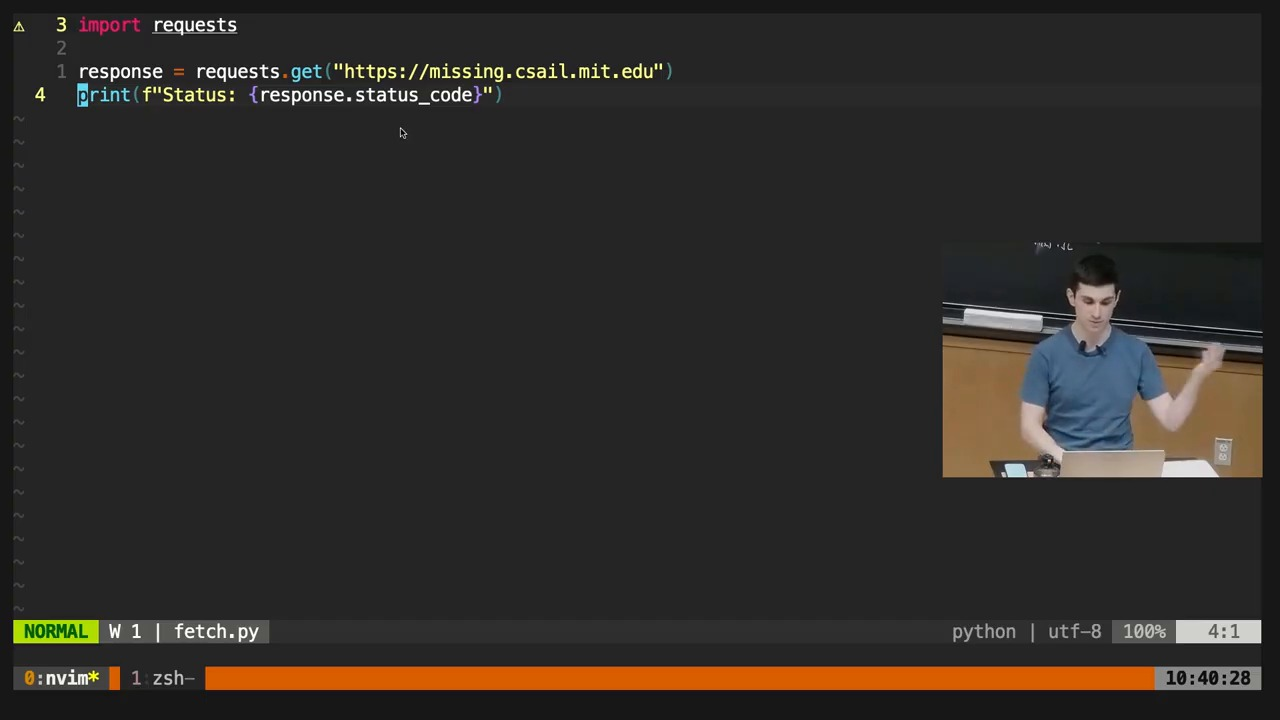
\includegraphics[width=0.92\textwidth]{figures/fig_01_requests_error.jpg}
\caption{只有两行的 Python 程序因为找不到 requests 模块而运行失败\vtag}
\end{figure}
\srcnote{00:02:15--00:02:30}
\end{minipage}


讲者展示了一个非常小的 Python 程序：导入 \texttt{requests} 库（用来发 HTTP 请求），然后下载课程网站。运行它会失败，失败原因编程语言运行时已经告诉我们了：\texttt{requests} 模块不存在。\texttt{requests} 不是 Python 默认安装的一部分，而是别人实现的，我们需要先把那份代码弄到电脑上才能使用。在 Python 里，随语言运行时一起提供的默认工具是 \texttt{pip}，执行 \texttt{pip install requests} 就表示我们要下载这个依赖。

\noindent\begin{minipage}{\textwidth}
\begin{figure}[H]
\centering
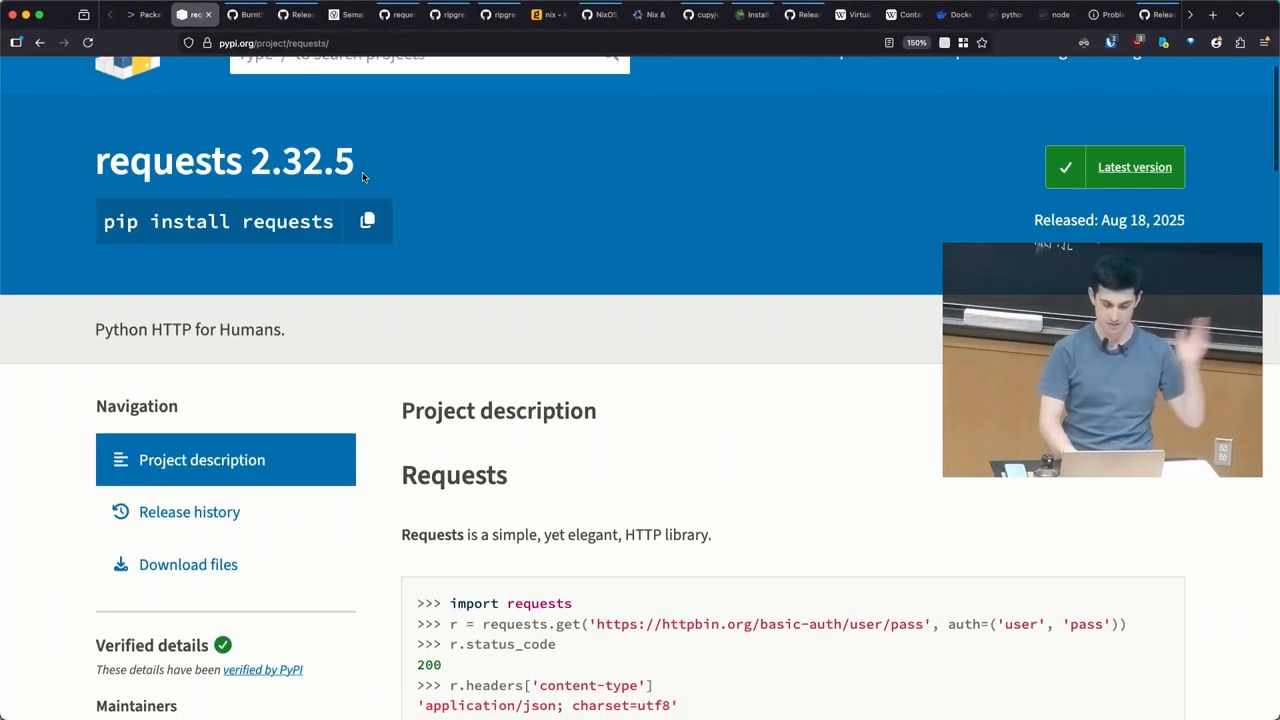
\includegraphics[width=0.92\textwidth]{figures/fig_02_pip_install.jpg}
\caption{PyPI 上的 requests 项目页，记录了安装它所需的全部信息\vtag}
\end{figure}
\srcnote{00:03:30--00:03:45}
\end{minipage}


讲者解释了 \texttt{pip} 打印出的那一大堆信息：我们请求 \texttt{requests} 包时，\texttt{pip} 去 Python 包索引（Python Package Index，PyPI）询问有没有这个包、能不能安装。PyPI 上确实有，并且存着安装所需的全部信息。但在安装 \texttt{requests} 之前，\texttt{pip} 还下载了别的库，那些是 \texttt{requests} 的依赖。安装一个包之前，要递归地遍历它的所有依赖、依赖的依赖，在整棵依赖树中按顺序把它们安装到文件系统里。

\noindent\begin{minipage}{\textwidth}
\begin{figure}[H]
\centering
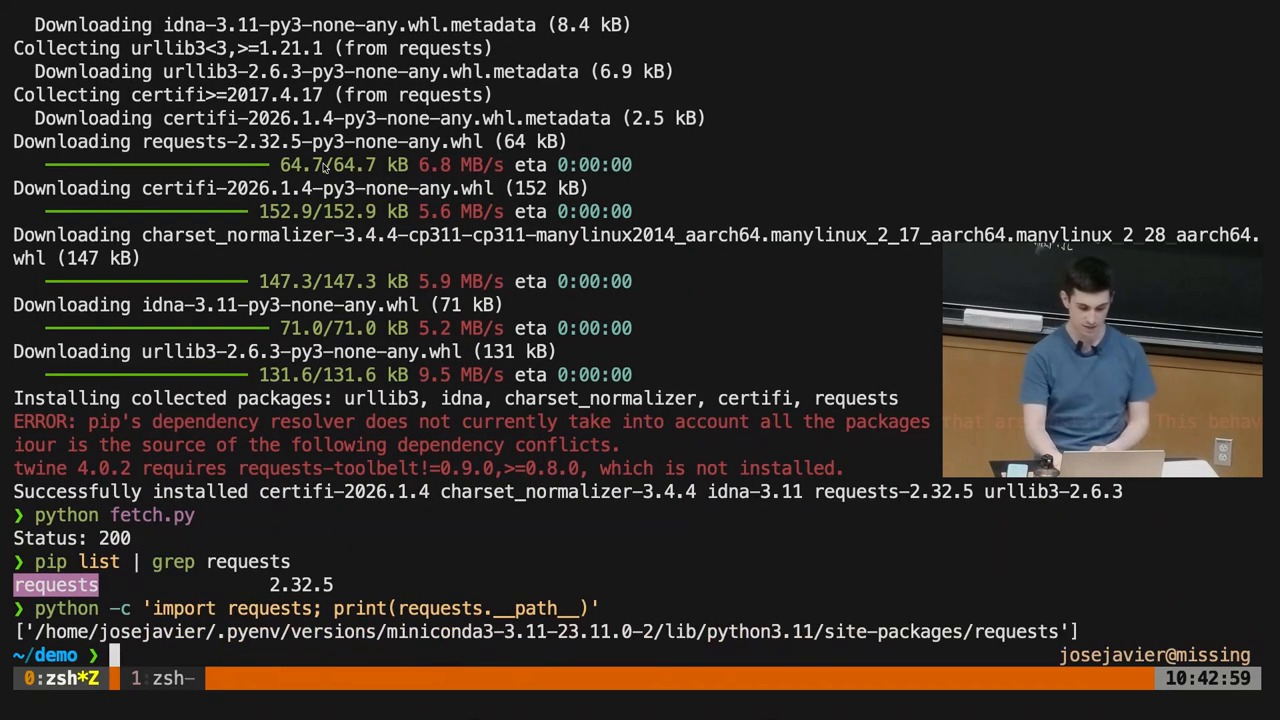
\includegraphics[width=0.92\textwidth]{figures/fig_03_pip_show.jpg}
\caption{用 \texttt{requests.\_\_path\_\_} 查看包被解压到了默认 Python 安装的哪个目录\vtag}
\end{figure}
\srcnote{00:04:45--00:05:00}
\end{minipage}


装好以后程序就能运行了，它成功下载了网页，打印出的 200 是 HTTP 状态码，表示一切顺利。用 \texttt{pip list} 可以确认装上的是 PyPI 上列出的最新版本；在 Python 里还能查看这个包被装到了哪里：它进入了默认的 Python 安装目录，从 PyPI 下载的那些文件都被解压在那里。

\subsection{不同语言，不同哲学}

讲者说，这个过程对 Python 是这样，换一种语言、换一种环境就会变化，而且变的不只是用哪个程序。例如 Rust 用 Cargo，它是一个统一的工具，编译、打包、发布几乎全都包办，是一条非常统一的工具链；而 Python 的统一发生在规范层面：语言规定好规则，至于工具由谁来写都可以，\texttt{pip} 只是完成这项工作的工具之一，还有其他遵循相同规则的竞争工具。

还有更极端的例子：如果你在电脑上装过 LaTeX，会发现有些发行版自带成千上万个包，你很少需要单独安装一个 LaTeX 包，因为对 LaTeX 来说，把所有东西都和语言一起打包是一种合理的模式。

\subsection{依赖冲突}

\noindent\begin{minipage}{\textwidth}
\begin{figure}[H]
\centering
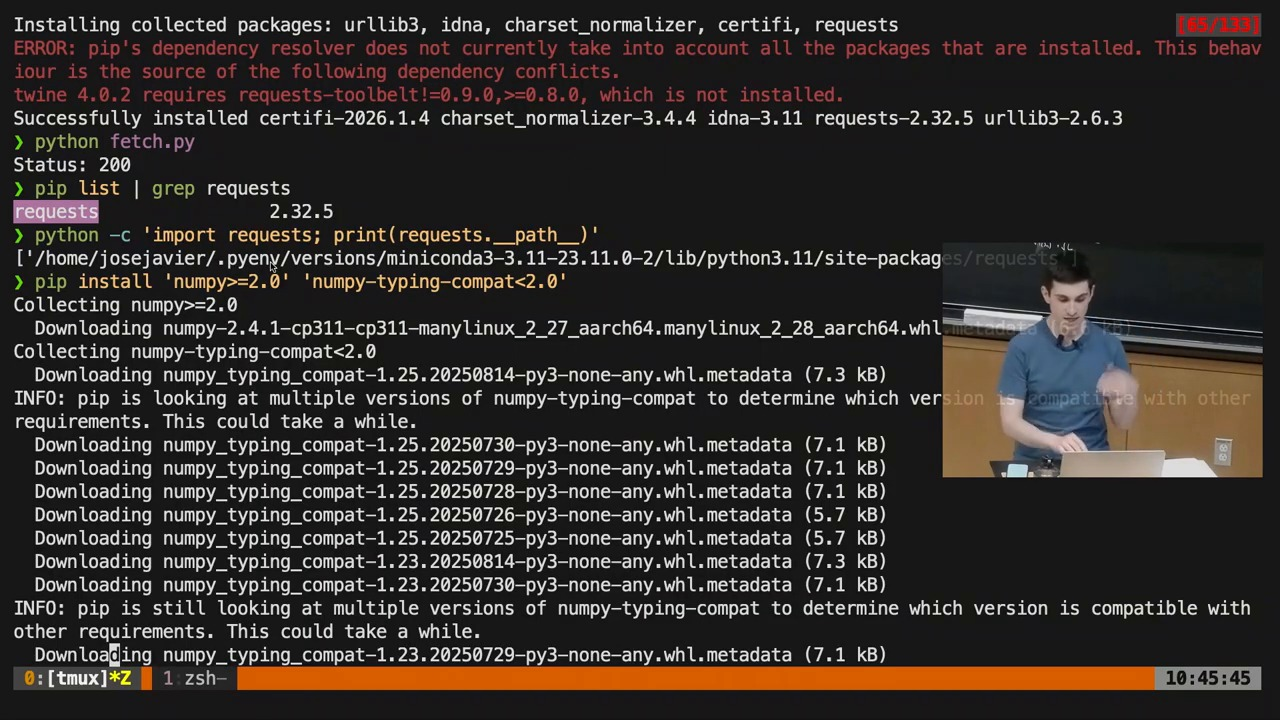
\includegraphics[width=0.92\textwidth]{figures/fig_04_conflict.jpg}
\caption{要求 numpy 不低于 2.0 而另一个库要求低于 2.0，解析器报告无解\vtag}
\end{figure}
\srcnote{00:07:30--00:07:45}
\end{minipage}


依赖越来越多时，就可能遇到依赖冲突。讲者构造了一个例子：要求 NumPy 的版本大于 2.0，同时安装一个 NumPy 的“兄弟库”，而它要求 NumPy 低于 2.0。执行后输出了很多信息，概括起来就是：不存在一组彼此兼容的版本，因为那个类型库要求 NumPy 低于 2.0。讲者承认这是个有点刻意的例子，但随着包越来越多，你可能真的会遇到无法让操作系统中所有 Python 包和谐共存的情况。

\begin{importantbox}{依赖是一棵树}
你声明的只是直接依赖，但安装时要满足的是整棵依赖树。任何两个包对同一个底层库提出互不相容的版本要求，整个安装就无解。这正是后面虚拟环境、版本约束和锁文件要解决的问题。
\end{importantbox}

\section{虚拟环境与运行时版本}

\subsection{venv}

\noindent\begin{minipage}{\textwidth}
\begin{figure}[H]
\centering
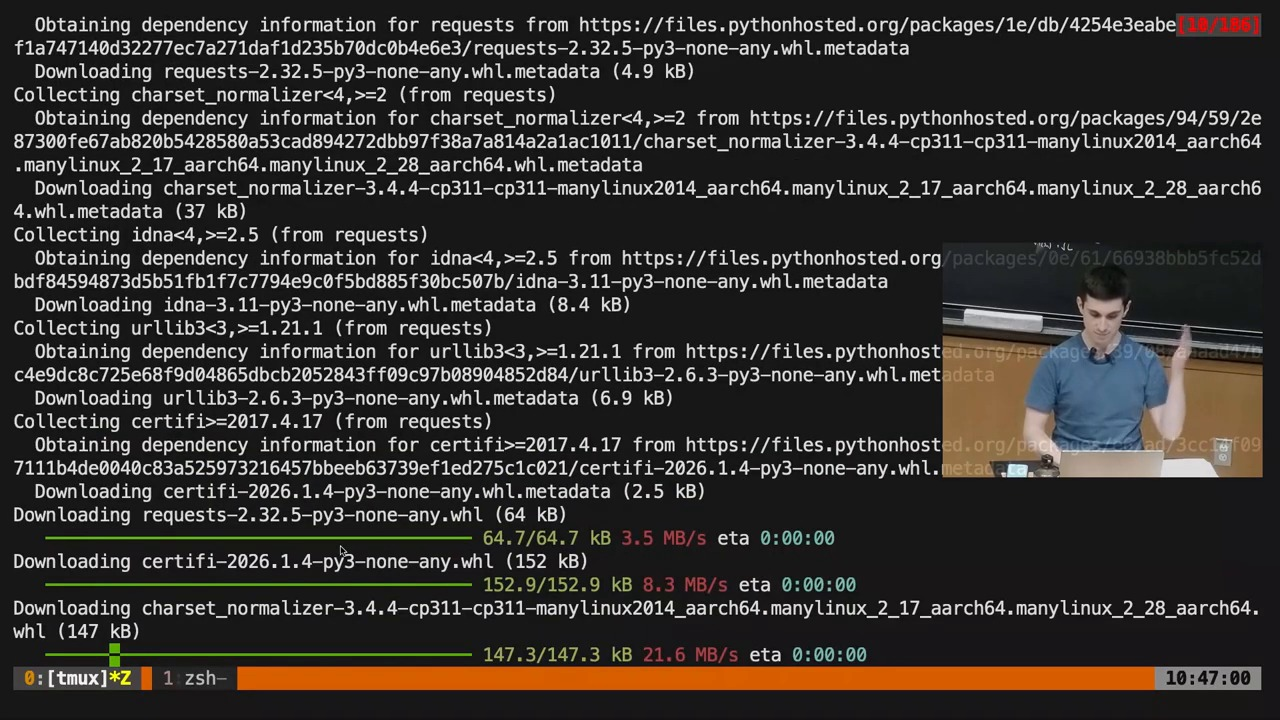
\includegraphics[width=0.92\textwidth]{figures/fig_05_venv.jpg}
\caption{在激活的 \texttt{myenv} 虚拟环境里重新安装 requests 及其依赖\vtag}
\end{figure}
\srcnote{00:08:45--00:09:00}
\end{minipage}


解决办法是使用环境。在 Python 里用 \texttt{python -m venv myenv} 创建环境：Python 会创建一份全新的、隔离的语言运行时副本。激活之后再查看 \texttt{python} 可执行文件的位置，它已经指向我们刚创建的 \texttt{myenv} 文件夹，与 Python 运行时相关的其他程序，比如 \texttt{pip}，也一样。此时再检查刚才装过的 \texttt{requests}，它不在了，因为它装在默认安装里，而这是一个隔离的环境。在这里同样可以安装它，过程几乎一样，同样会解析所有依赖；\texttt{pip list} 显示除了默认的 setuptools 和 pip，还有这些依赖；查看安装位置，它现在位于自己的隔离环境中。

讲者说，一般来说，为每个项目建一个环境来存放依赖是很好的做法。随着项目越来越多，这样更容易追踪每个项目的确切依赖，也不容易陷入通常所说的依赖地狱（dependency hell），也就是出现大量难以解决的依赖冲突。

\subsection{uv}

\noindent\begin{minipage}{\textwidth}
\begin{figure}[H]
\centering
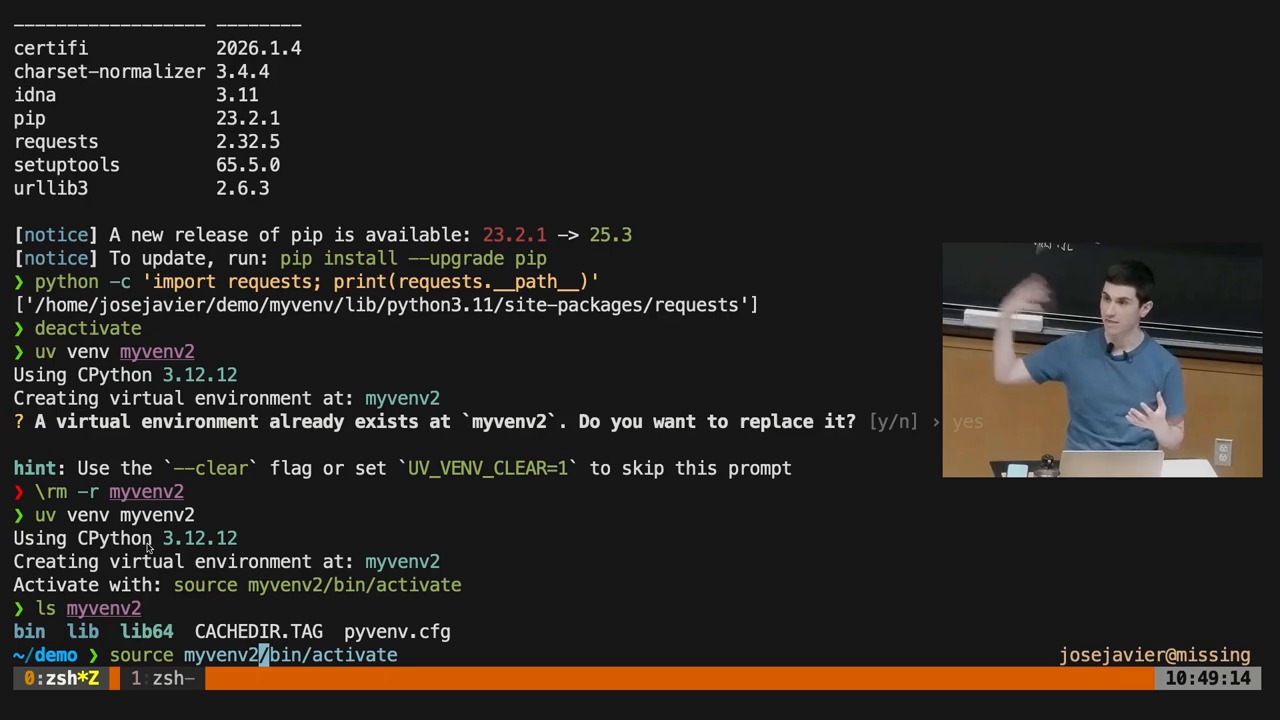
\includegraphics[width=0.92\textwidth]{figures/fig_06_uv_venv.jpg}
\caption{用 uv 创建虚拟环境并安装 requests，速度明显快于 pip\vtag}
\end{figure}
\srcnote{00:11:00--00:11:15}
\end{minipage}


讲者说，Python 的打包生态相当复杂，多年来不断演变，有多个工具实现了同样的打包逻辑。如今最容易上手的是 \texttt{uv}，它不只是 \texttt{pip} 的替代品，而是一次替代了好几个工具，后面的例子都会用它。它更易用，人们最常称道的是它比 \texttt{pip} 快得多，不只是安装，依赖解析等很多操作都快。

\texttt{uv} 也能创建虚拟环境。讲者强调，虚拟环境并没有什么魔法，它只是另一个文件夹，里面有一堆对应一个 Python 安装的文件。执行 \texttt{source} 命令时，我们只是在修改 Shell 里的 \texttt{PATH} 等环境变量，让 \texttt{python} 解析到另一个位置。用 \texttt{uv} 安装 \texttt{requests}，做的事完全一样，但快得多；包越来越大时，可以从几分钟缩短到几秒钟。

\begin{lstlisting}[language=bash]
uv venv
source .venv/bin/activate
uv pip install requests
\end{lstlisting}

\subsection{隔离运行时版本}

\noindent\begin{minipage}{\textwidth}
\begin{figure}[H]
\centering
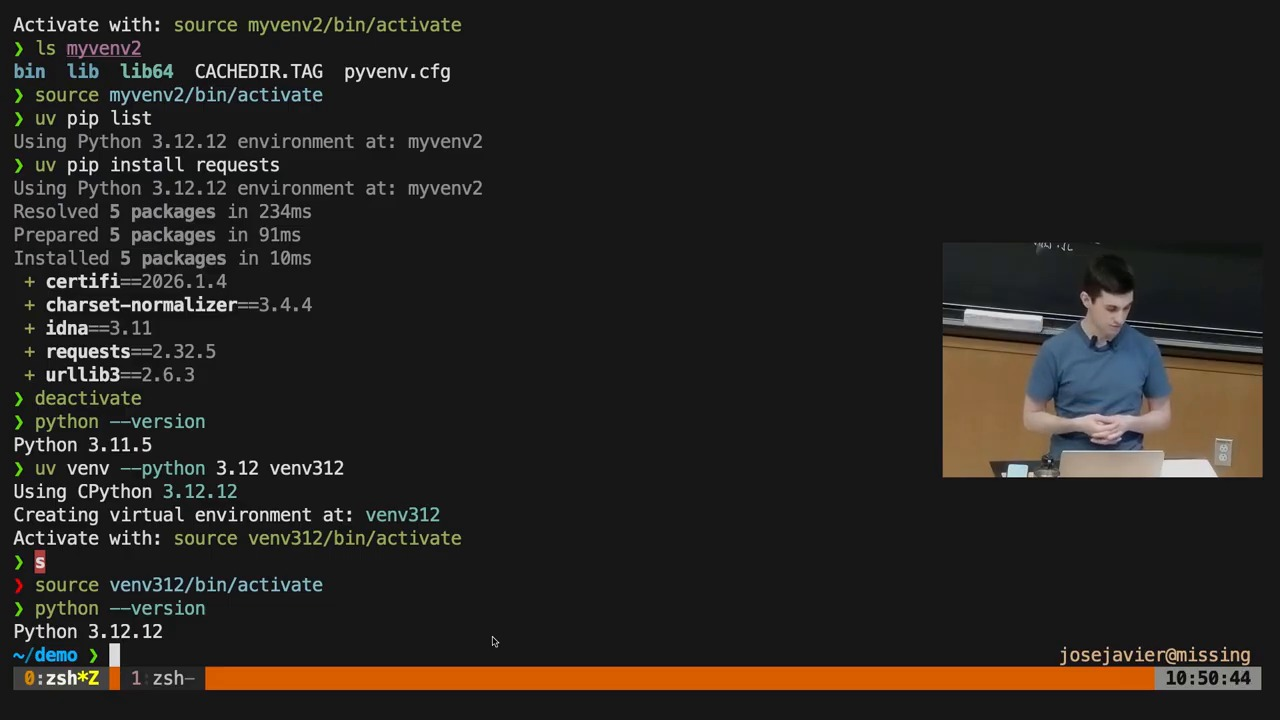
\includegraphics[width=0.92\textwidth]{figures/fig_07_py312.jpg}
\caption{指定 Python 3.12 创建虚拟环境，激活后版本随之改变\vtag}
\end{figure}
\srcnote{00:12:30--00:12:45}
\end{minipage}


除了隔离依赖，另一个常见模式（不只在 Python 中）是隔离语言运行时的版本。讲者的电脑上装的是 3.11，创建的环境默认也是 3.11；如果项目使用 3.12，可以创建一个指定 Python 版本的虚拟环境，激活后可以看到版本确实变成了 3.12。这是依赖隔离的另一部分。

\begin{knowledgebox}{激活环境到底做了什么}
讲义作者补充：\texttt{source .venv/bin/activate} 只是把 \texttt{.venv/bin} 放到 \texttt{PATH} 最前面，并设置 \texttt{VIRTUAL\_ENV} 等变量，这正好对应第一讲讲的“Shell 按 \texttt{PATH} 顺序查找程序”。忘记激活环境是新手最常见的错误之一，讲者在后面的演示中就遇到了一次。
\end{knowledgebox}

\subsection{本章小结}

依赖由包管理器从包索引递归下载；全局安装容易冲突，所以每个项目使用一个虚拟环境，必要时连运行时版本一起隔离。接下来反过来：怎样让别人安装我们的代码。

\section{把自己的代码做成包}

\subsection{为什么换个目录就找不到了}

\noindent\begin{minipage}{\textwidth}
\begin{figure}[H]
\centering
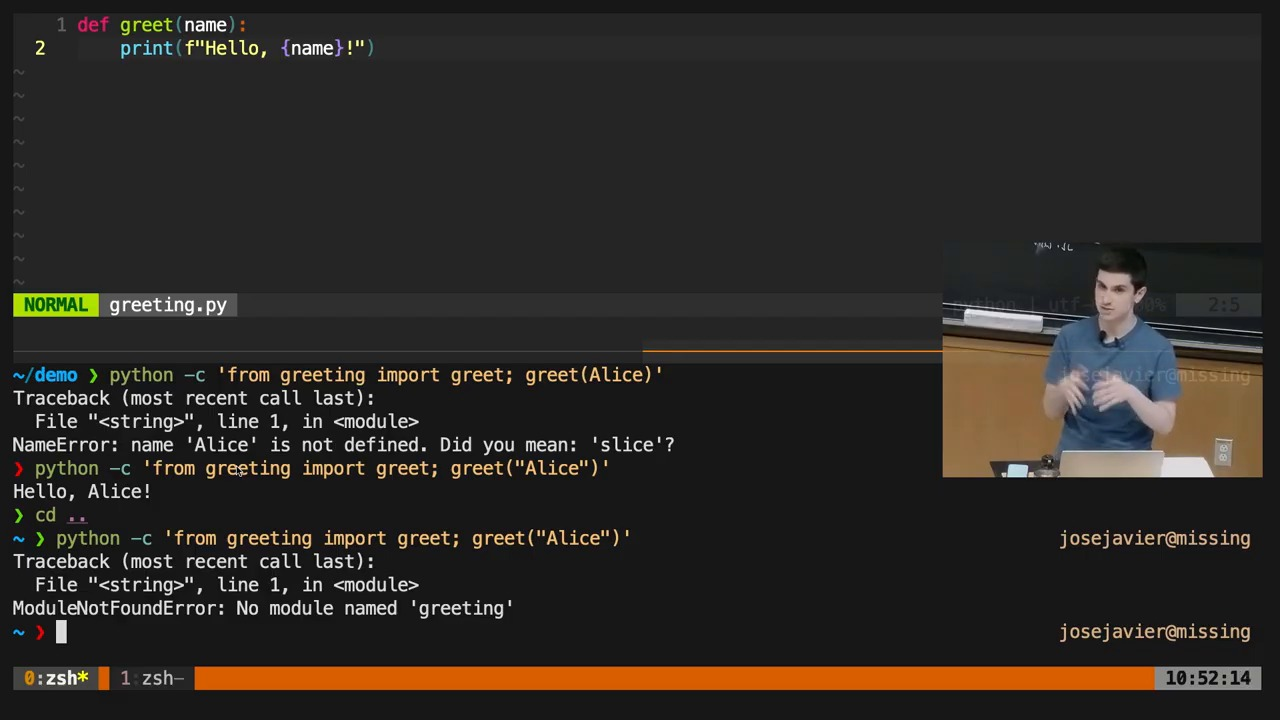
\includegraphics[width=0.92\textwidth]{figures/fig_08_greet_local.jpg}
\caption{在同一目录下能导入 greeting，换一个目录就报 ModuleNotFoundError\vtag}
\end{figure}
\srcnote{00:14:00--00:14:15}
\end{minipage}


讲者写了一个文件 \texttt{greeting.py}，里面是最简单的 Hello World 函数。在同一个文件夹里 \texttt{from greeting import greet} 能工作，因为 Python 默认会在当前运行的文件夹里查找匹配的文件。但换一个文件夹再做同样的事就失败了：Python 没有办法找到这个 \texttt{greeting} 包，它不是当前安装的一部分。要让包可安装，就要遵守 Python 的规则。

\subsection{pyproject.toml}

\noindent\begin{minipage}{\textwidth}
\begin{figure}[H]
\centering
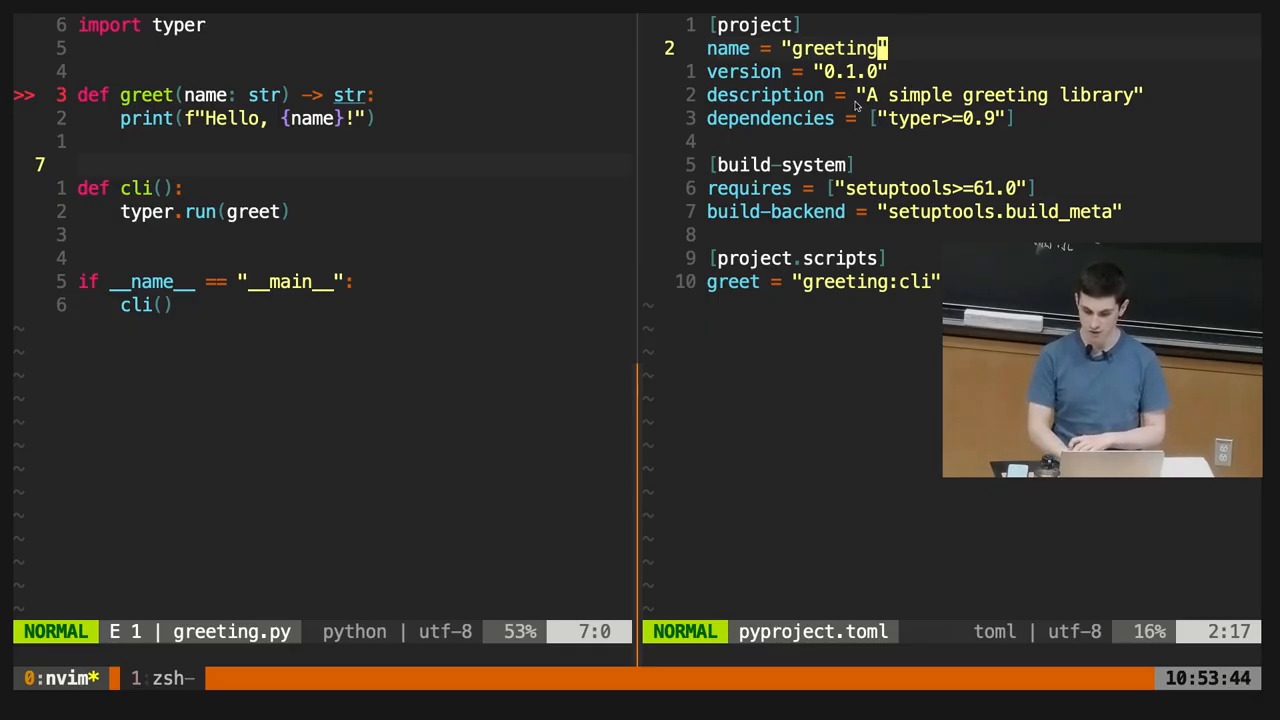
\includegraphics[width=0.92\textwidth]{figures/fig_09_pyproject.jpg}
\caption{左边是加入 Typer 命令行入口的 greeting.py，右边是声明包信息的 pyproject.toml\vtag}
\end{figure}
\srcnote{00:15:30--00:15:45}
\end{minipage}


右边的示例中代码基本相同，只是加了一个命令行入口，使用的是 Typer 库，和标准库的 \texttt{argparse} 类似，这里用它主要是为了引入一个依赖。右边的 \texttt{pyproject.toml} 就是游戏规则：Python 告诉你，想创建一个别人能安装的包，就要按特定模式写这样一个文件。讲者说你可能见过 \texttt{requirements.txt}、\texttt{setup.py} 等其他方式，它们也能用，但今后推荐的是这种方式。

\begin{lstlisting}[language=Python]
[project]
name = "greeting"
version = "0.1.0"
description = "A simple greeting library"
dependencies = ["typer>=0.9"]

[build-system]
requires = ["setuptools>=61.0"]
build-backend = "setuptools.build_meta"

[project.scripts]
greet = "greeting:cli"
\end{lstlisting}

讲者逐项解释：\texttt{name} 是包名，安装后 Python 靠它找到这个包；\texttt{version} 是版本，可用于约束版本；然后是描述；\texttt{dependencies} 声明所有依赖，这里表示没有安装 0.9 或更高版本的 Typer 就不能安装这个库；\texttt{build-system} 指定用来构建制品的构建系统；最后一部分告诉 Python，安装时还要创建一个名为 \texttt{greet} 的程序，它调用 \texttt{greeting} 文件里的 \texttt{cli} 函数。

\noindent\begin{minipage}{\textwidth}
\begin{figure}[H]
\centering
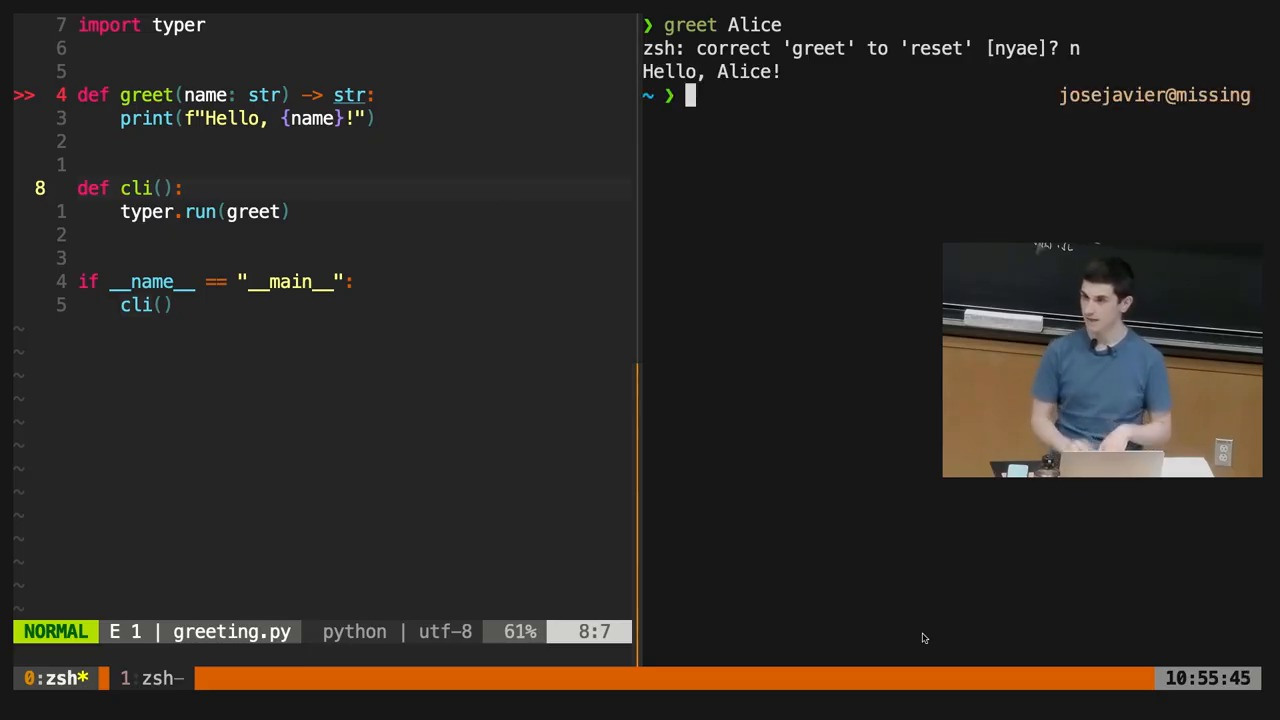
\includegraphics[width=0.92\textwidth]{figures/fig_10_installed.jpg}
\caption{安装后在任意目录都能导入 greeting，命令行里也多了一个 greet 命令\vtag}
\end{figure}
\srcnote{00:17:30--00:17:45}
\end{minipage}


有了这些，执行 \texttt{uv pip install .}，它解析了整个依赖并构建了包。讲者第一次尝试时忘了激活环境，激活之后，环境里不仅装上了我们的包，还装上了它的所有依赖。现在在任何地方导入 \texttt{greeting} 都能成功，包列表里能找到版本 0.1 的 \texttt{greeting}，而且多了一个 \texttt{greet} 命令，这是因为我们从这个文件夹里的源文件构建了这个包。

\section{源码与预编译制品}

\subsection{源码不等于制品}

\noindent\begin{minipage}{\textwidth}
\begin{figure}[H]
\centering
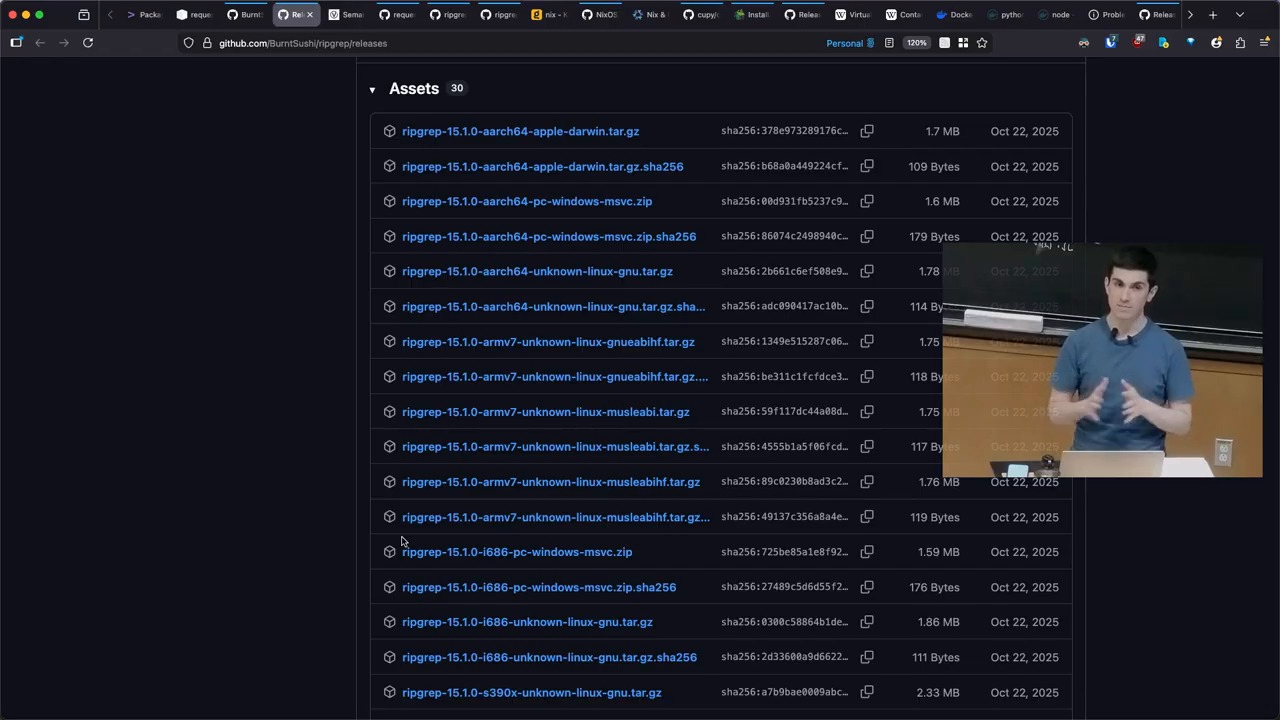
\includegraphics[width=0.92\textwidth]{figures/fig_11_ripgrep_bins.jpg}
\caption{ripgrep 发布页按操作系统和 CPU 架构提供了一长串预编译二进制\vtag}
\end{figure}
\srcnote{00:19:00--00:19:15}
\end{minipage}


讲者指出，上面的做法意味着别人要安装这个包，就需要我们的全部文件。实际的软件打包中，通常要区分源代码和预构建的制品（预编译二进制）。源代码只是构建一切的原始指令，要使用它，你可能需要一整条工具链和各种依赖库；而真正运行程序，可能并不需要那么多代码。

一个好例子是之前讲过的 ripgrep：它有一个发布页（releases），上面有许多预编译的二进制文件，下载其中一个，应该就能直接在电脑上执行。代价是：预编译之后，能运行这个软件的平台就受到了限制。最常见的两个维度是操作系统和 CPU 架构，所以发布页上不止一个文件，而是一长串。Windows PC、运行 Apple Silicon 的 macOS、树莓派上的 Linux，各自需要对应架构的二进制。

\subsection{wheel}

\noindent\begin{minipage}{\textwidth}
\begin{figure}[H]
\centering
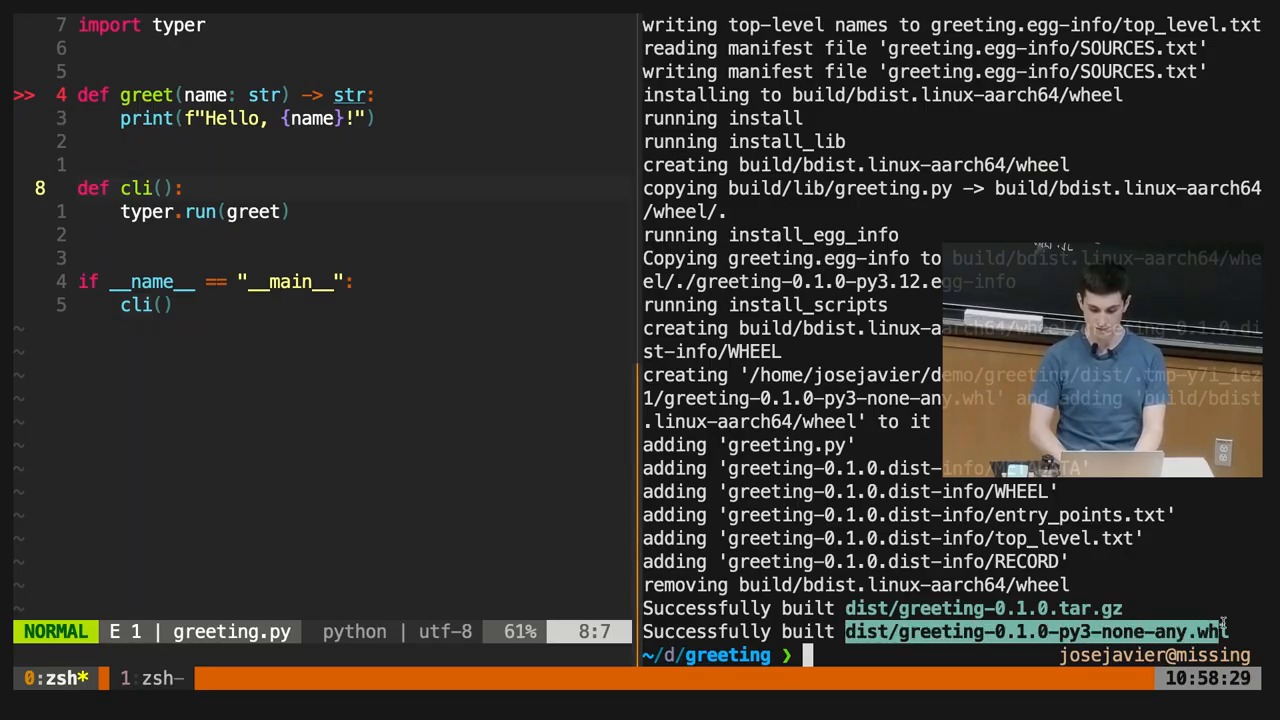
\includegraphics[width=0.92\textwidth]{figures/fig_12_wheel_build.jpg}
\caption{\texttt{uv build} 生成一个源码包和一个 wheel 文件\vtag}
\end{figure}
\srcnote{00:20:15--00:20:30}
\end{minipage}


回到 Python，构建别人可用的制品的方式是创建 wheel，wheel 只是一种格式。执行 \texttt{uv build} 会产生很多输出，Python 以标准化的方式打包我们的应用，使 \texttt{pip}、\texttt{uv} 等工具都能正确地管理和安装它。它生成了两个文件：第一个包含源代码，第二个是 wheel 文件。把这个单独的文件交给别人，他们用 \texttt{pip install} 加上文件名就能安装，我们演示时就从这一个文件装上了同一个库。

\noindent\begin{minipage}{\textwidth}
\begin{figure}[H]
\centering
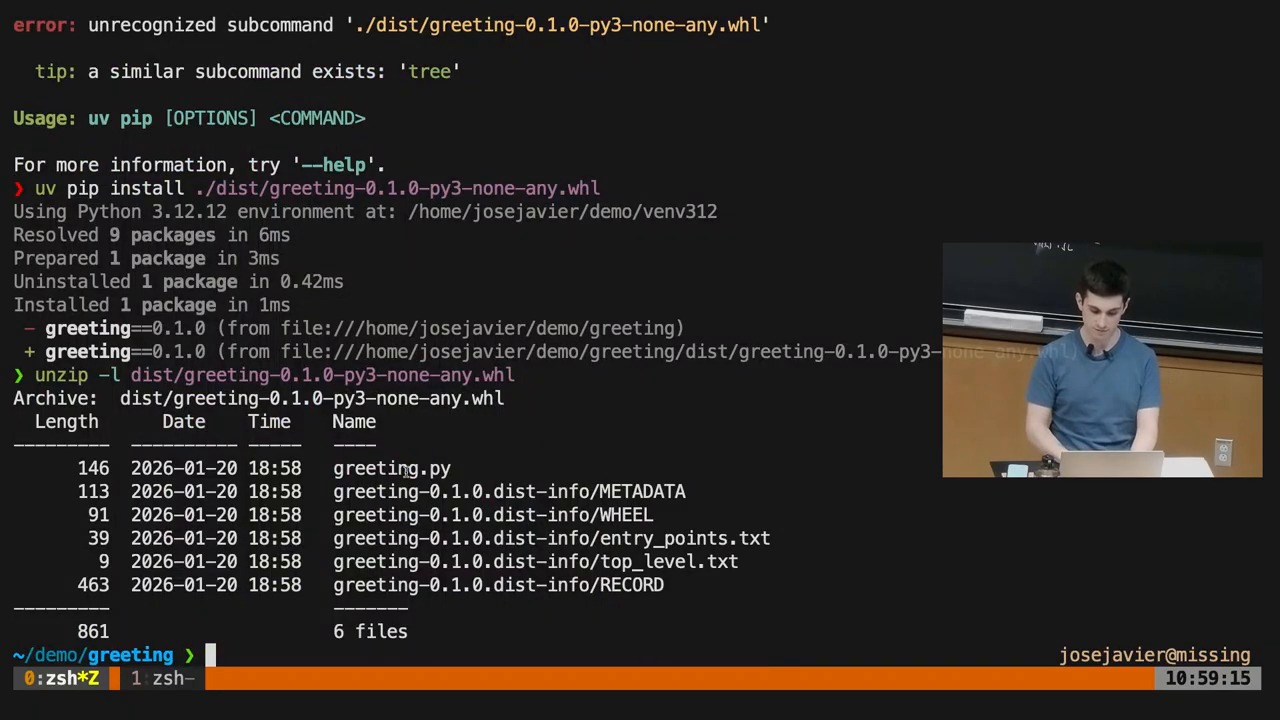
\includegraphics[width=0.92\textwidth]{figures/fig_13_wheel_zip.jpg}
\caption{wheel 本质上是一个 zip，里面只有 greeting.py 和几份元数据\vtag}
\end{figure}
\srcnote{00:21:00--00:21:15}
\end{minipage}


讲者强调 wheel 文件也没有魔法：在 Python 中它就是一个 zip 压缩包。因为我们的包很小，这个 zip 里只有我们写的 \texttt{greeting} 文件，以及包管理器需要的几个元数据文件。

\begin{knowledgebox}{sdist 与 wheel}
讲义作者补充：\texttt{uv build} 生成的两个文件分别是源码分发包（sdist，\texttt{.tar.gz}）和构建好的分发包（wheel，\texttt{.whl}）。纯 Python 包的 wheel 文件名里带有 \texttt{py3-none-any}，表示与平台无关；含 C 扩展的包则要为每个平台、每个 Python 版本分别构建 wheel，后面的 CuPy 就是这种情况。
\end{knowledgebox}

\section{版本与可复现性}

\subsection{版本约束}

\noindent\begin{minipage}{\textwidth}
\begin{figure}[H]
\centering
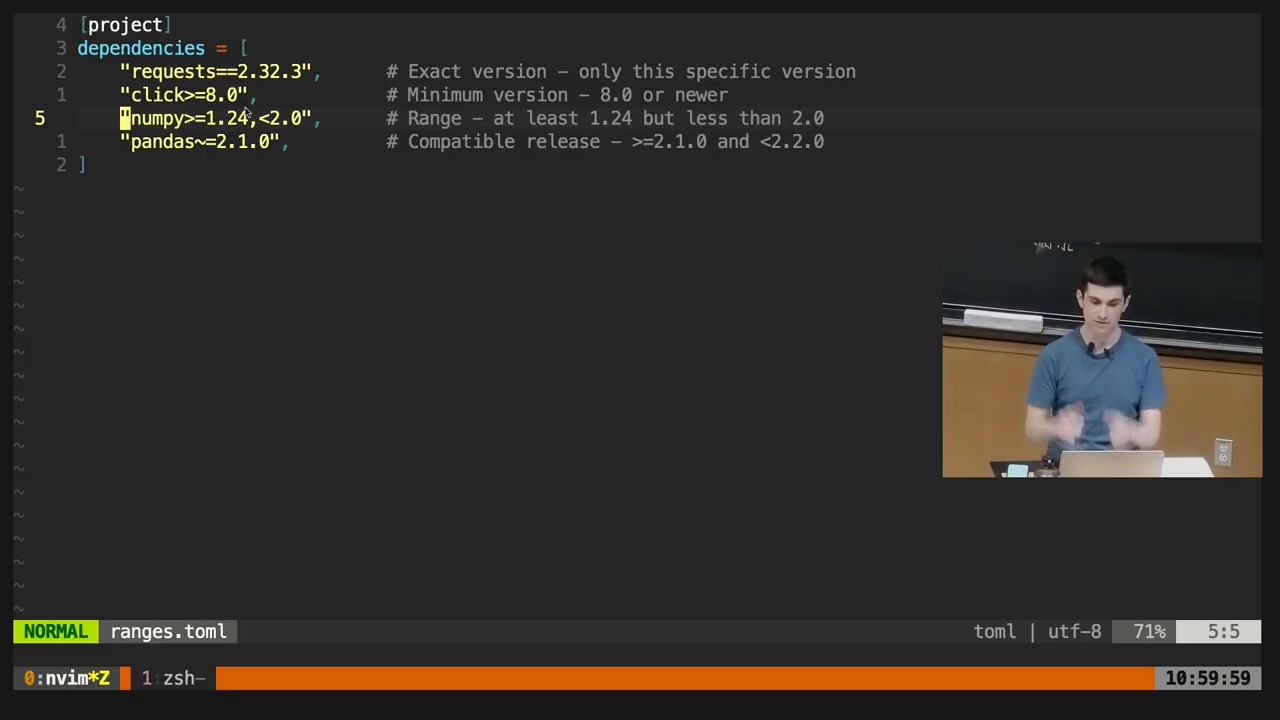
\includegraphics[width=0.92\textwidth]{figures/fig_14_version_spec.jpg}
\caption{版本说明符示例：精确版本、最低版本、范围以及兼容版本\vtag}
\end{figure}
\srcnote{00:21:45--00:22:00}
\end{minipage}


随着库越来越大，依赖越来越多，一个挑战是：要声明依赖，就得知道它们能和你的代码一起工作。软件打包中的做法是声明哪些版本范围可行、哪些不行。语法因语言略有不同，但可以表达：要这个确切版本；至少这个版本；更受限的，比如大于等于某个版本但永远不到 2.0。

\begin{lstlisting}[language=Python]
[project]
dependencies = [
    "requests==2.32.3",  # Exact version - only this specific version
    "click>=8.0",        # Minimum version - 8.0 or newer
    "numpy>=1.24,<2.0",  # Range - at least 1.24 but less than 2.0
    "pandas~=2.1.0",     # Compatible release - >=2.1.0 and <2.2.0
]
\end{lstlisting}

人们发布新版本时，用户通常不会安装最新的版本，而是安装已知稳定的版本。回到 ripgrep 的例子，它发布了 15.0.0、15.1.0 等版本，并说明了变化：修了一个 bug，宣布了一个新特性。这叫变更日志（changelog），是人们报告相对上一版有什么变化、能否放心升级的方式。原则上，你可以把所有依赖的变更日志都读一遍。

\noindent\begin{minipage}{\textwidth}
\begin{figure}[H]
\centering
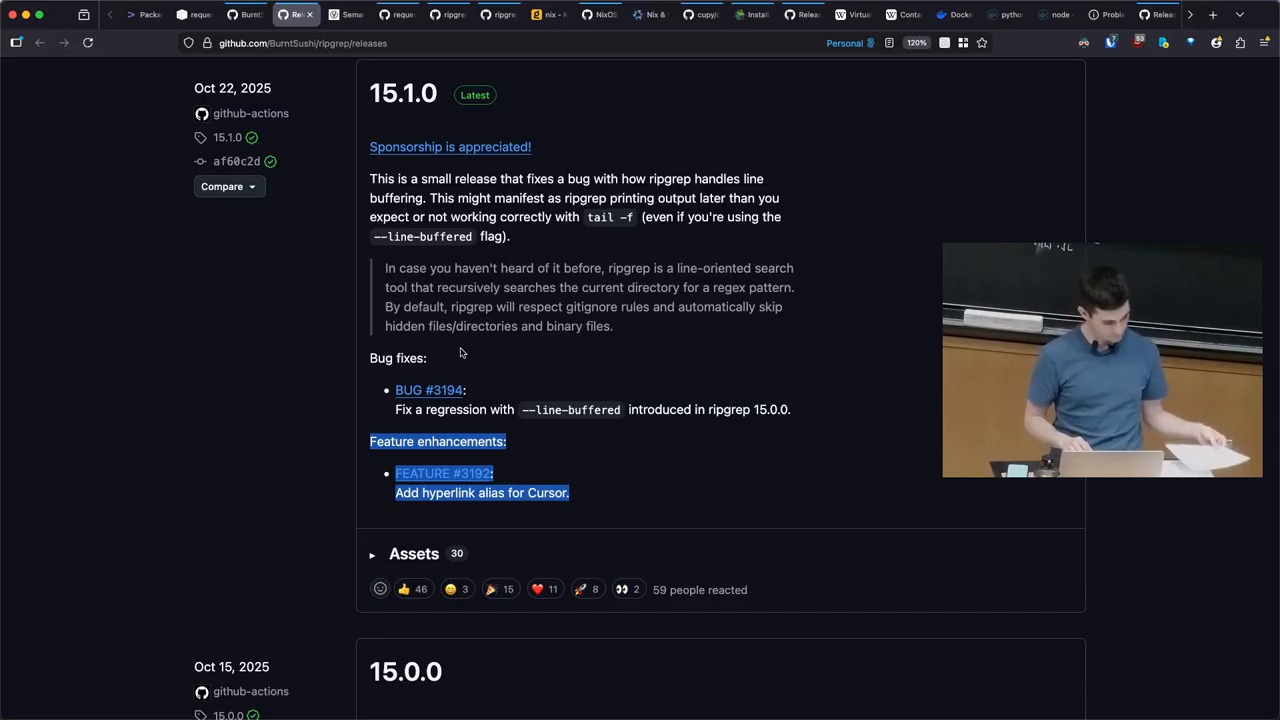
\includegraphics[width=0.92\textwidth]{figures/fig_15_changelog.jpg}
\caption{ripgrep 15.1.0 的变更日志列出了新特性和缺陷修复\vtag}
\end{figure}
\srcnote{00:25:00--00:25:15}
\end{minipage}


问题在于，这不只是你的依赖，还有依赖的依赖的依赖。即使在我们这个最小的例子里，用 \texttt{uv tree} 查看依赖树，只加了一个 Typer，它实际上就依赖了很多其他库。

\subsection{语义化版本}

\noindent\begin{minipage}{\textwidth}
\begin{figure}[H]
\centering
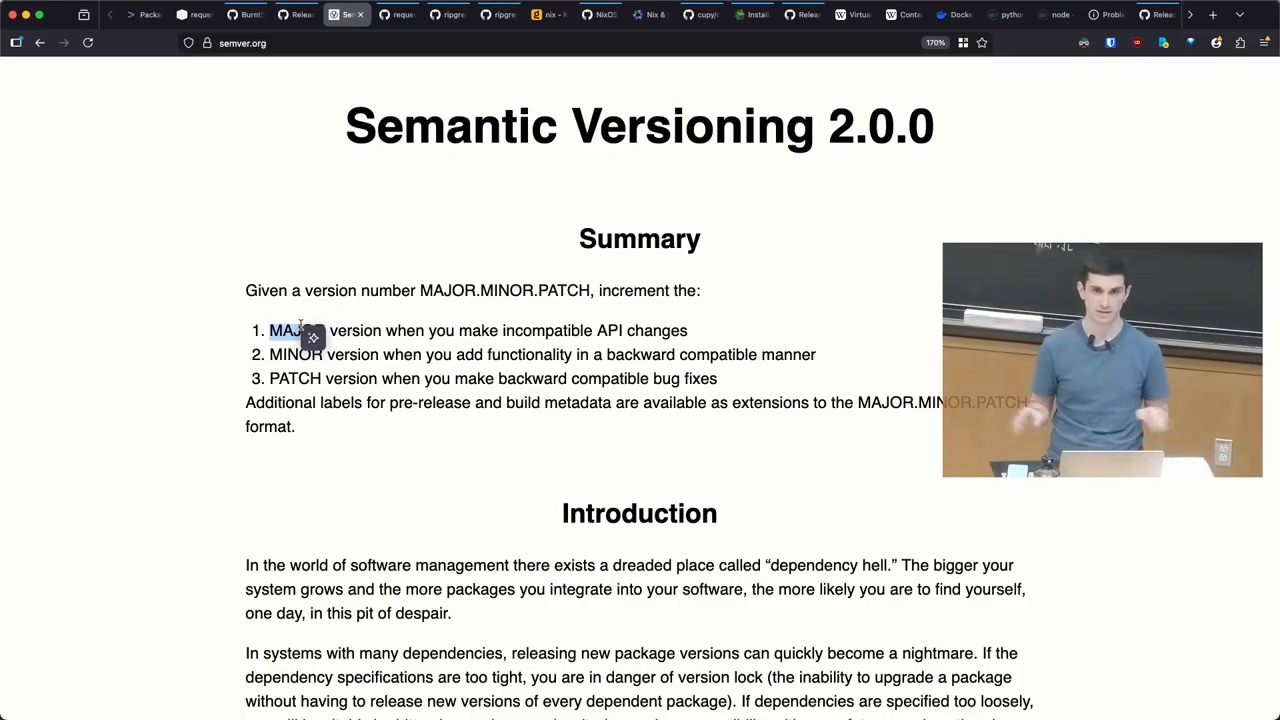
\includegraphics[width=0.92\textwidth]{figures/fig_16_semver.jpg}
\caption{语义化版本 2.0.0 规范：主版本、次版本、修订号各有含义\vtag}
\end{figure}
\srcnote{00:24:00--00:24:15}
\end{minipage}


于是软件开发者形成了约定：以某种方式增加版本号意味着什么。最流行的约定叫语义化版本（semantic versioning）。版本有三个数字，都是自然数，分别是主版本号（major）、次版本号（minor）和修订号（patch），它们说明相对上一版改变了什么：
\begin{itemize}
\item 升级主版本号时，基本不提供任何保证，之前能用的东西升级后可能坏掉，所以你会看到那种禁止主版本变化的约束；
\item 升级次版本号表示有新特性，但之前能用的一切仍然应该能用，只是新特性只在这个版本里才有；
\item 只有缺陷修复、也许还有文档改动时，通常只升级修订号，对库的用户来说一切和以前完全一样。
\end{itemize}

ripgrep 和很多库一样遵循语义化版本：它从 15.0.0 升到 15.1.0，就是因为加了新特性。

\begin{warningbox}{约定不是保证}
讲义作者提醒：语义化版本是人的承诺而不是机器的检查，次版本升级偶尔也会意外破坏兼容性；另外按照规范，主版本号为 0 的阶段（例如 0.9）表示 API 尚不稳定，任何升级都可能带来不兼容的变化。这正是需要锁文件的原因之一。
\end{warningbox}

\subsection{库与应用：范围还是钉死}

\noindent\begin{minipage}{\textwidth}
\begin{figure}[H]
\centering
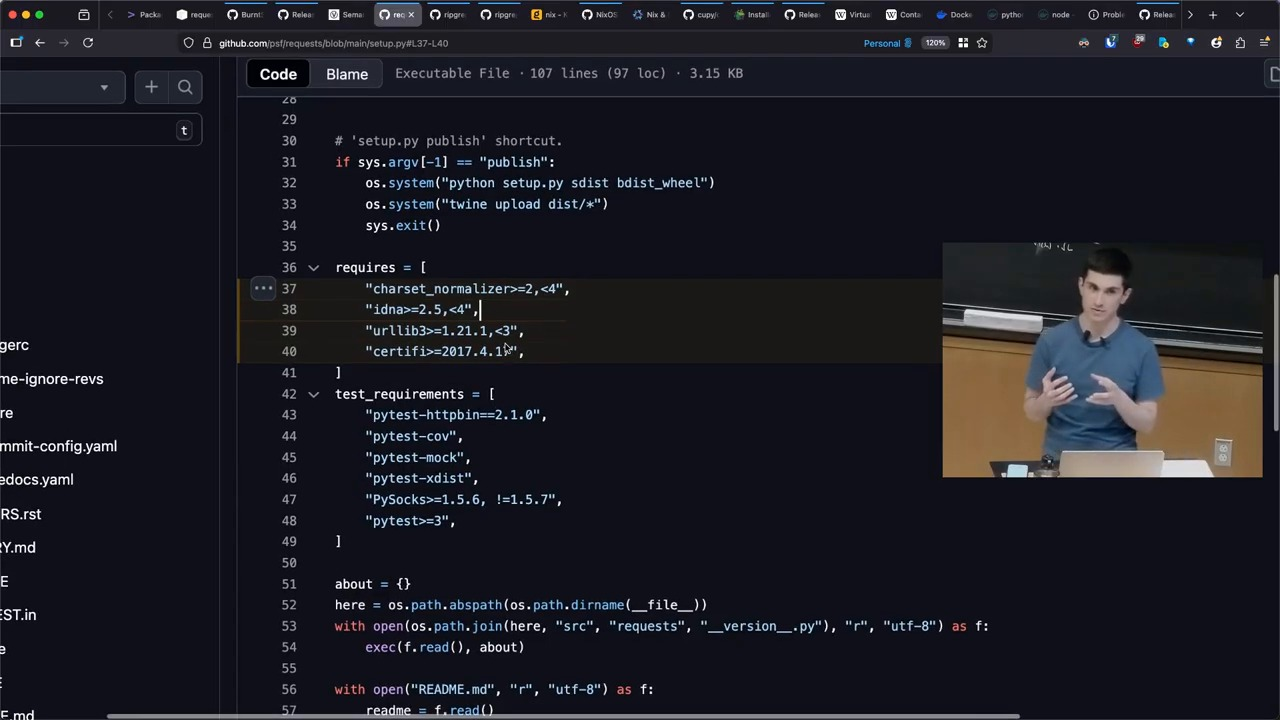
\includegraphics[width=0.92\textwidth]{figures/fig_17_requests_deps.jpg}
\caption{requests 的打包脚本只给出宽松的版本范围，基本只约束主版本\vtag}
\end{figure}
\srcnote{00:26:30--00:26:45}
\end{minipage}


讲者接着讲版本的另一面：构建应用时，存在一种张力：一边是把所有版本都精确指定，这样别人装到的就是你用的确切版本，不会出问题；另一边是只给范围，希望在这些版本上都能用。这取决于你构建的程序类型。如果你在构建一个库，比如 \texttt{requests}，在 Python 中就应该给出宽范围，因为别人会把 \texttt{requests} 和许多其他库装在一起，如果要求过严，就很可能让人陷入依赖冲突，没法把我们的库和其他库一起装。看 \texttt{requests} 怎样声明依赖就能看到这一点：它给出了三个宽范围，大多只约束主版本，以防万一。

如果你构建的是供人使用的应用，给出宽范围就没有任何好处，我们要把一切都钉死，让最终产品的使用者得到可复现的体验。看 ripgrep 的依赖，它没有给出任何范围，每个依赖都必须使用确切版本来构建这个工具，因为他们测试过这些版本能一起工作。

\begin{importantbox}{经验法则}
库：声明宽松的版本范围，把选择权留给最终用户，避免制造冲突。应用：钉死每一个版本（最好连同间接依赖和校验和一起写进锁文件），保证每次构建、每台机器得到的都是测试过的那一组版本。
\end{importantbox}

\subsection{锁文件}

\noindent\begin{minipage}{\textwidth}
\begin{figure}[H]
\centering
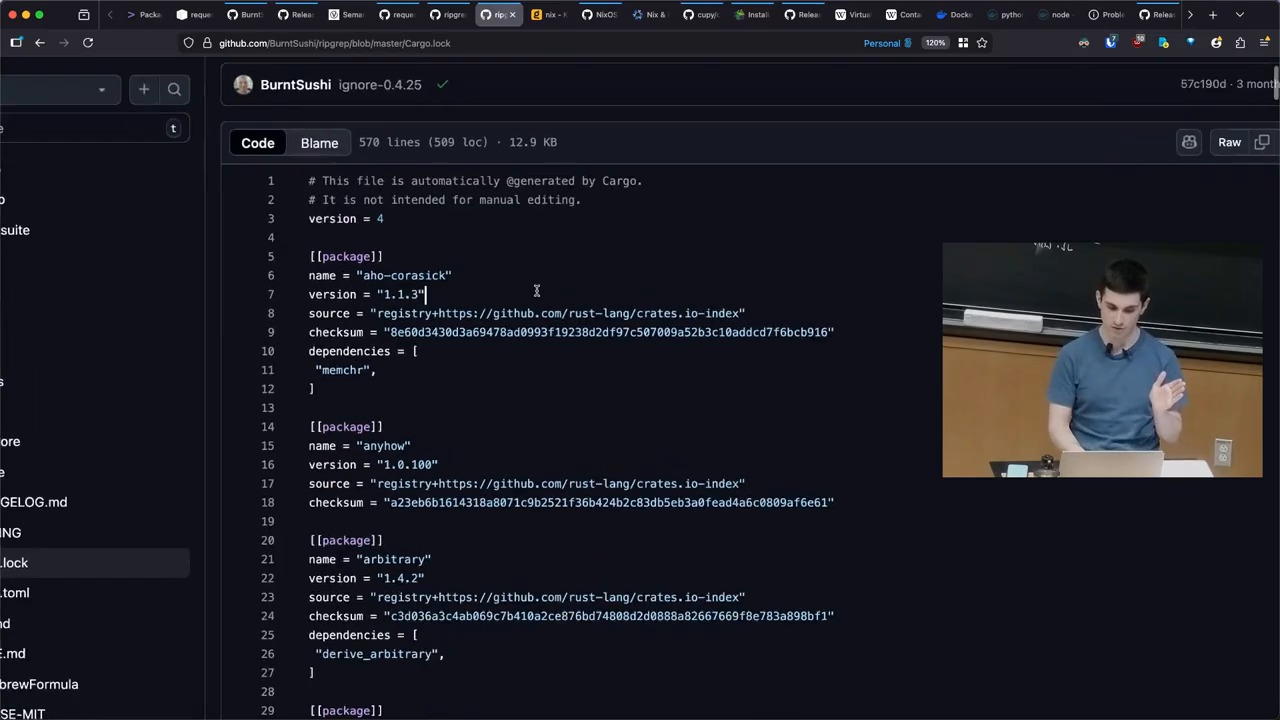
\includegraphics[width=0.92\textwidth]{figures/fig_18_cargo_lock.jpg}
\caption{Cargo 生成的锁文件记录了每个间接依赖的确切版本和校验和\vtag}
\end{figure}
\srcnote{00:27:30--00:27:45}
\end{minipage}


随着人们试图让打包更可复现，不只是指定版本，而是更彻底地指定几乎一切。讲者展示了 Cargo 包管理器生成的一个文件，它不仅解析了依赖，还解析了依赖的依赖，为每一个都记录了确切版本和这个库的校验和（checksum）：也就是说，不只是“这个版本”，而是“我们下载它时，这个文件的哈希是这个值”。

\noindent\begin{minipage}{\textwidth}
\begin{figure}[H]
\centering
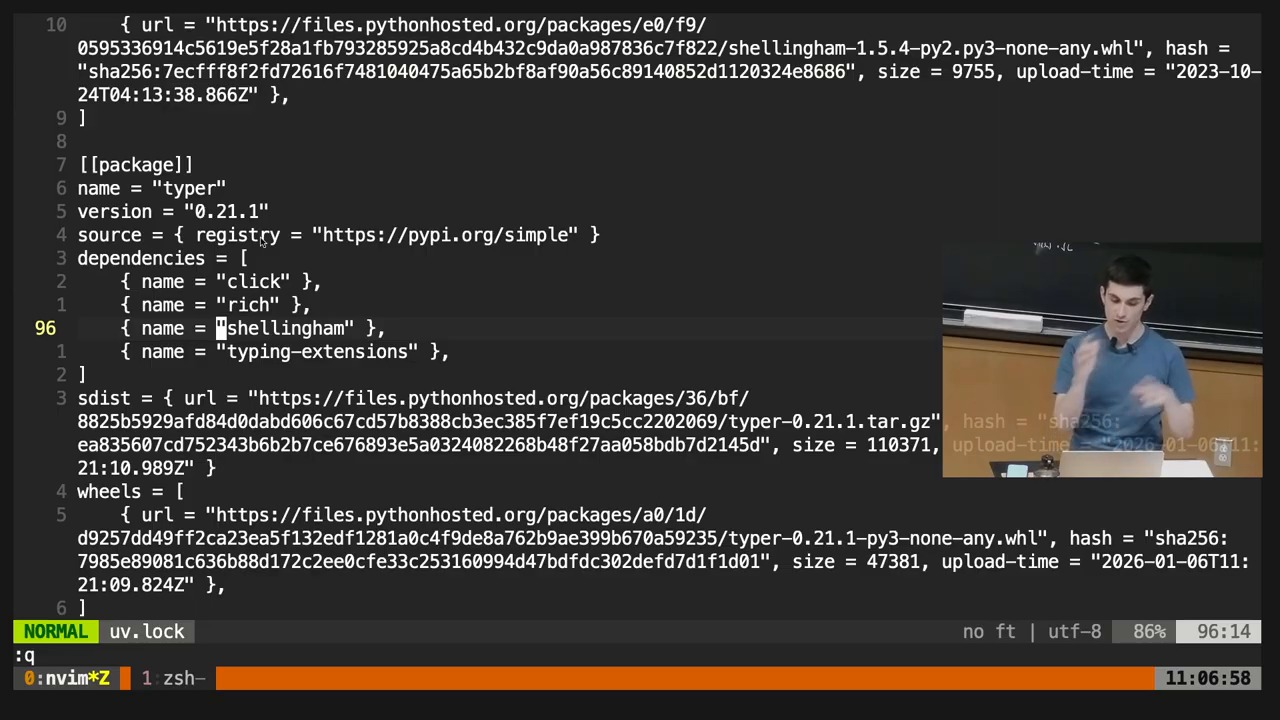
\includegraphics[width=0.92\textwidth]{figures/fig_19_uv_lock.jpg}
\caption{uv.lock 中 Typer 被解析为 0.21.1，并附有下载地址和哈希\vtag}
\end{figure}
\srcnote{00:28:45--00:29:00}
\end{minipage}


在 Python 里也能做同样的事。在我们的包目录里执行 \texttt{uv lock}，会生成一个锁文件，包含大量元数据，它是给机器读的而不是给人读的，但我们可以查看。例如我们说 Typer 必须大于 0.9，而在生成这个可复现配置时，它用的是最新的 0.21.1；而且它把源码和 wheel 都下载了，并记录了从哪里下载、下载的文件的确切哈希。此后任何人使用 \texttt{uv sync}，都会得到完全相同的版本。如果他们只用 \texttt{pyproject.toml}，也许现在有了更新的 Typer，就会装上新版；而用 \texttt{uv sync}，就保证得到我们测试应用时的那一组版本。

\subsection{语言之外：Nix}

讲者说，这种做法当然有局限。和打包中的大多数事情一样，一旦越过编程语言环境的边界，就得使用面向更广泛依赖管理的工具。对于更复杂的管理，有 Nix 这样的包管理器，它不只处理 Python，而是处理你能安装的所有包，为操作系统中的一切提供可复现的方式。你也许觉得只要是 3.12 就行，但 Python 需要 C 编译器来构建，而 C 编译器的版本可能不同。Nix 就是管理电脑里每一点可变性的方式，甚至有一个基于这一思想的操作系统，你会用灵活性换取复杂性；但值得知道，在可复现性至关重要的场合，有这样的工具可用。

\subsection{本章小结}

版本约束表达“哪些版本可行”，语义化版本让版本号携带含义；库给范围、应用钉死；锁文件连同哈希记录整棵依赖树。可是有些依赖根本不在语言包管理器的管辖之内。

\section{虚拟机与容器}

\subsection{语言管不了的依赖}

\noindent\begin{minipage}{\textwidth}
\begin{figure}[H]
\centering
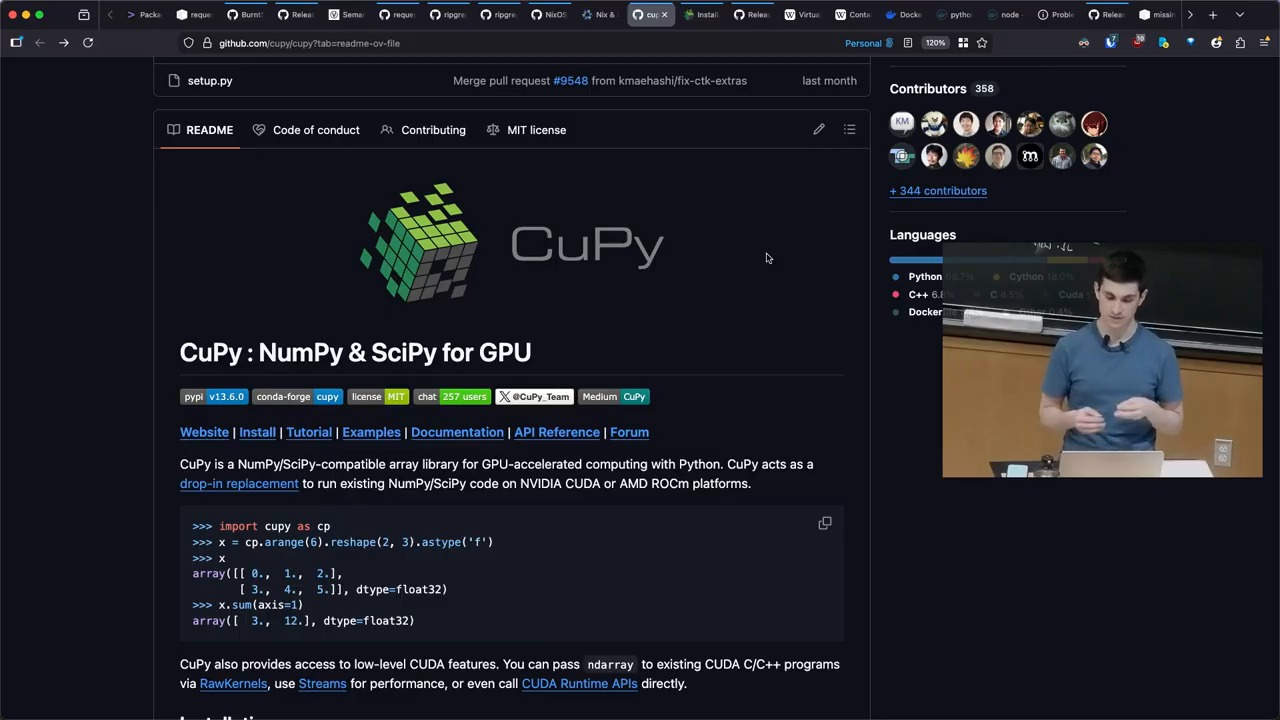
\includegraphics[width=0.92\textwidth]{figures/fig_20_cupy.jpg}
\caption{CuPy 的安装说明要求先装好兼容的 CUDA 工具包\vtag}
\end{figure}
\srcnote{00:31:00--00:31:15}
\end{minipage}


讲者举例：在 Python 中开始依赖编程语言运行时之外的东西，比如 GPU 驱动。CuPy 是一个 Python 包装层，用来调用一堆 CUDA，也就是 NVIDIA 的指令，而这些是 Python 无法管理的。CuPy 的安装说明不是简单地说“\texttt{pip install} 就行”，而是要求你已经装好兼容的 CUDA 工具包。我们不可能在 Python 打包中声明这一点，必须往上走一层。

\noindent\begin{minipage}{\textwidth}
\begin{figure}[H]
\centering
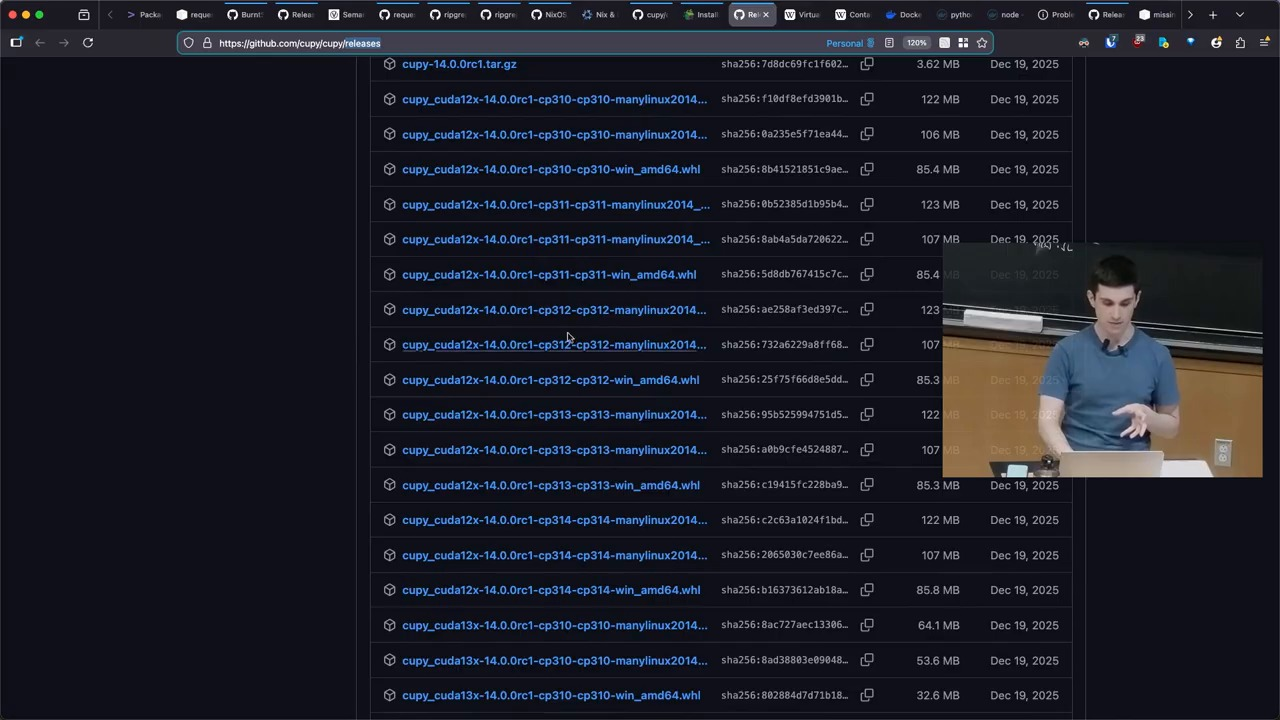
\includegraphics[width=0.92\textwidth]{figures/fig_21_cupy_wheels.jpg}
\caption{CuPy 为不同 CUDA 版本、Python 版本和平台分别构建了 wheel\vtag}
\end{figure}
\srcnote{00:32:30--00:32:45}
\end{minipage}


看 CuPy 怎样打包它的 Python wheel，能看到和 ripgrep 一样的模式：ripgrep 只有操作系统和 CPU 架构两个维度，CuPy 仍然有这两个，比如 Windows 和 AMD64；但因为它与 Python 和 CUDA 的许多特性绑在一起，还得为不同的 CUDA 运行时、不同的 Python 版本（比如 3.12、3.10）分别编译，你需要找到正确的制品才能安装。为了避免这些复杂性，我们真正想要的是：在制品里附带用户可能需要的一切。

\subsection{从虚拟机到容器}

\noindent\begin{minipage}{\textwidth}
\begin{figure}[H]
\centering
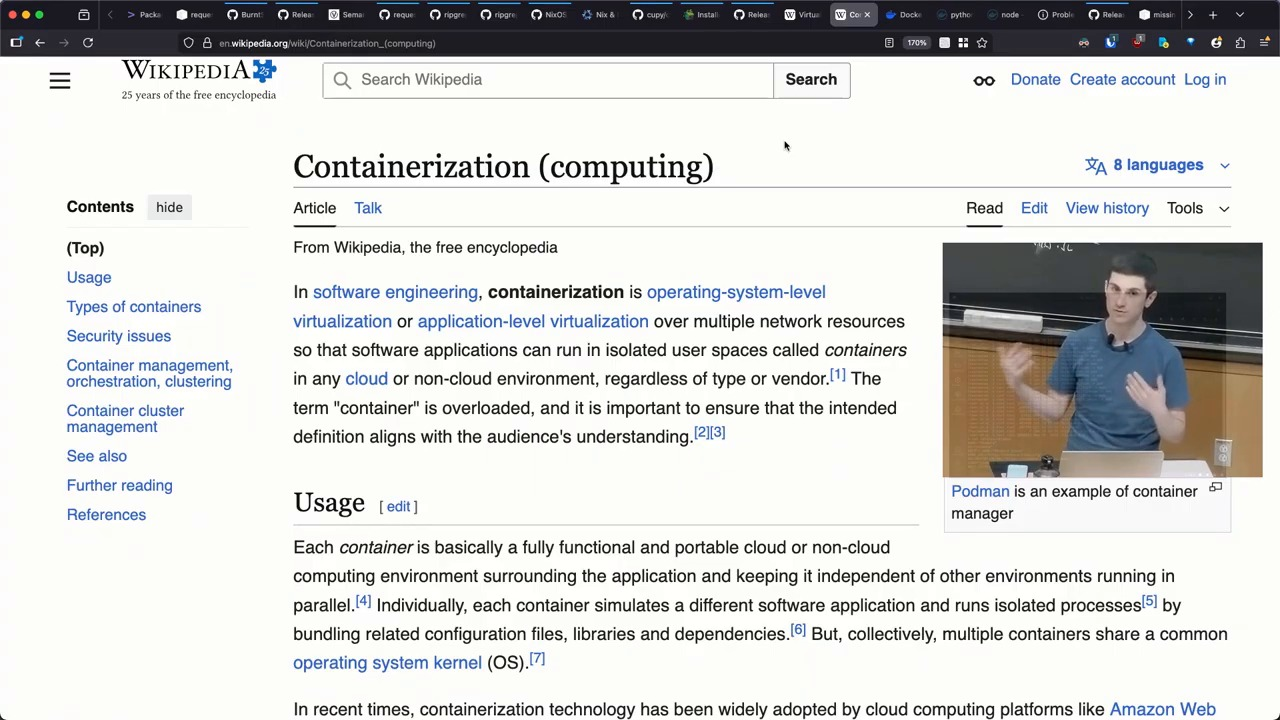
\includegraphics[width=0.92\textwidth]{figures/fig_22_containers.jpg}
\caption{维基百科对容器化的解释：共享宿主内核，只隔离应用层\vtag}
\end{figure}
\srcnote{00:34:30--00:34:45}
\end{minipage}


问题是，那可能意味着把整台电脑打包发出去。怎么发出一整台电脑？传统上人们正是这么做的：虚拟化，在电脑里运行电脑，虽有一些限制，但大体可行，可以在 Windows 里运行 Linux，反之亦然。给你一个虚拟机镜像，你就能执行它，拥有程序需要的所有依赖。虚拟机的缺点是开销大：只为了运行一个应用，就要在机器里运行一整个操作系统。

为了权衡这一点，开发者意识到，大多数应用只关心用户态的依赖，不需要修改操作系统本身。于是可以复用操作系统的大量核心组件，只隔离应用层，这就是容器背后的思想。容器只在部分操作系统上原生支持，Linux 和 BSD 支持，Windows 上则没有这个概念；在 Windows 或 Mac 上运行容器时，实际上是先运行一个 Linux 虚拟机，再在里面运行容器。讲者说这没关系，因为生产环境中部署的大量应用用的就是 Linux，各种发行版而已，而且越来越多地采用容器模式。

容器有不同的实现，工具也随之不同。目前最流行的是 Docker，它依赖一个叫 containerd 的容器运行时，其他工具也与之兼容。如果你听说过 Kubernetes，它使用同样的方式来定义一台机器，而 Kubernetes 有容错等更多特性，却可以复用同样的镜像。

\begin{knowledgebox}{虚拟机与容器的区别}
讲义作者整理：虚拟机模拟完整硬件，每个虚拟机运行自己的内核，隔离强但开销大、启动慢；容器共享宿主机的内核，只隔离文件系统、进程、网络等用户态资源，轻量、秒级启动。镜像（image）是容器的模板，容器是镜像运行起来的实例。
\end{knowledgebox}

\subsection{运行一个容器}

\noindent\begin{minipage}{\textwidth}
\begin{figure}[H]
\centering
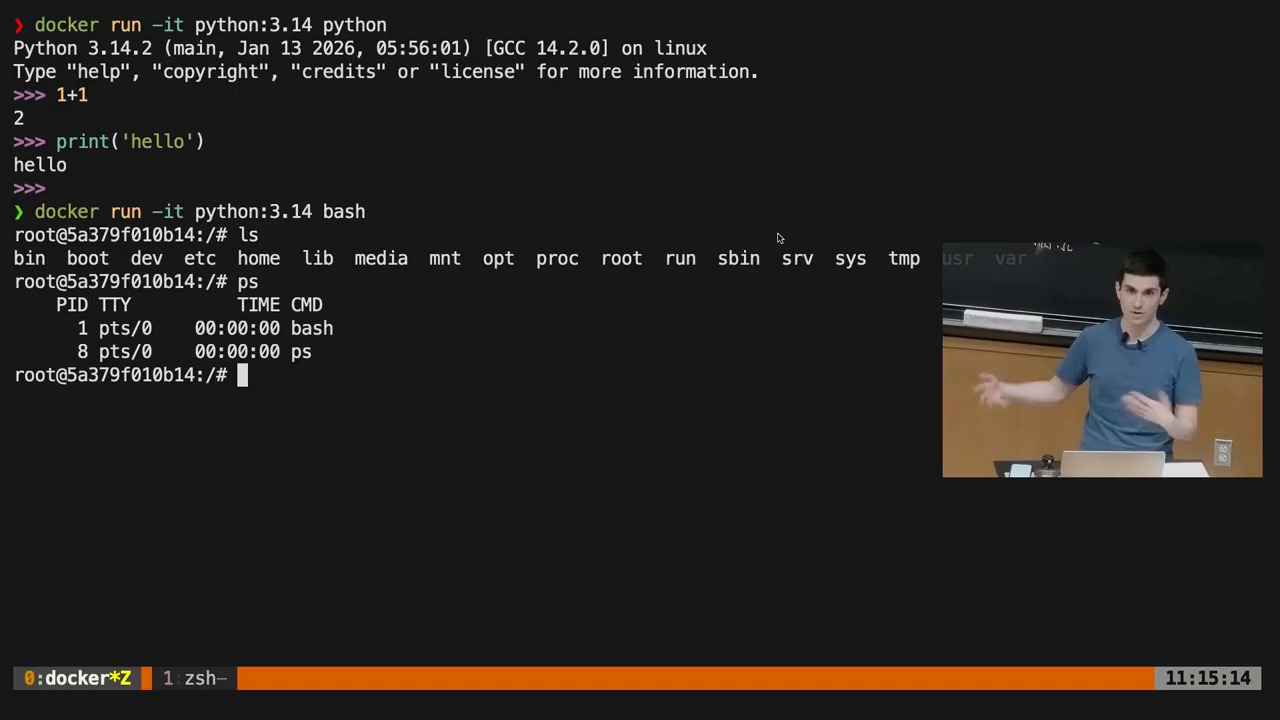
\includegraphics[width=0.92\textwidth]{figures/fig_23_docker_run.jpg}
\caption{在 python:3.14 容器里运行 bash，\texttt{ps aux} 只看到寥寥几个进程\vtag}
\end{figure}
\srcnote{00:37:00--00:37:15}
\end{minipage}


讲者说，讲了很多抽象概念，实际是什么样子？实际上你安装 Docker，它会启动一个进程，让你把操作系统的这部分能力复用给其他容器。执行 \texttt{docker run -it python:3.14 python}，\texttt{-it} 表示交互式，看起来就像直接运行 Python，你可以做平时做的任何事；但其实不同，这个 3.14 的 Python 运行在机器上一个隔离的容器里，它不是一个环境，而是被隔离出来的一整台机器。把 \texttt{python} 换成 \texttt{bash}，就能查看文件系统和正在运行的进程。由于容器没有操作系统簿记的那些开销，这里几乎没有进程，\texttt{ps aux} 显示的只有你自己启动的那些。

\texttt{python:3.14} 之所以是合法的容器镜像，是因为在 Docker Hub 上有人构建了这个官方镜像，它是某种 Linux。可以验证是哪种：它是 Debian 安装，Debian 是一个 Linux 发行版，上面装好了一个可用的 Python 运行时。如果需要别的工具链，比如 Node，思路相同，告诉 Docker 下载对应镜像即可。讲者提前下载好了这些镜像以免拖慢讲课，用 \texttt{docker images} 能看到几个镜像，都是从 Docker 服务器下载的。

\section{编写 Dockerfile}

\subsection{第一个 Dockerfile}

\noindent\begin{minipage}{\textwidth}
\begin{figure}[H]
\centering
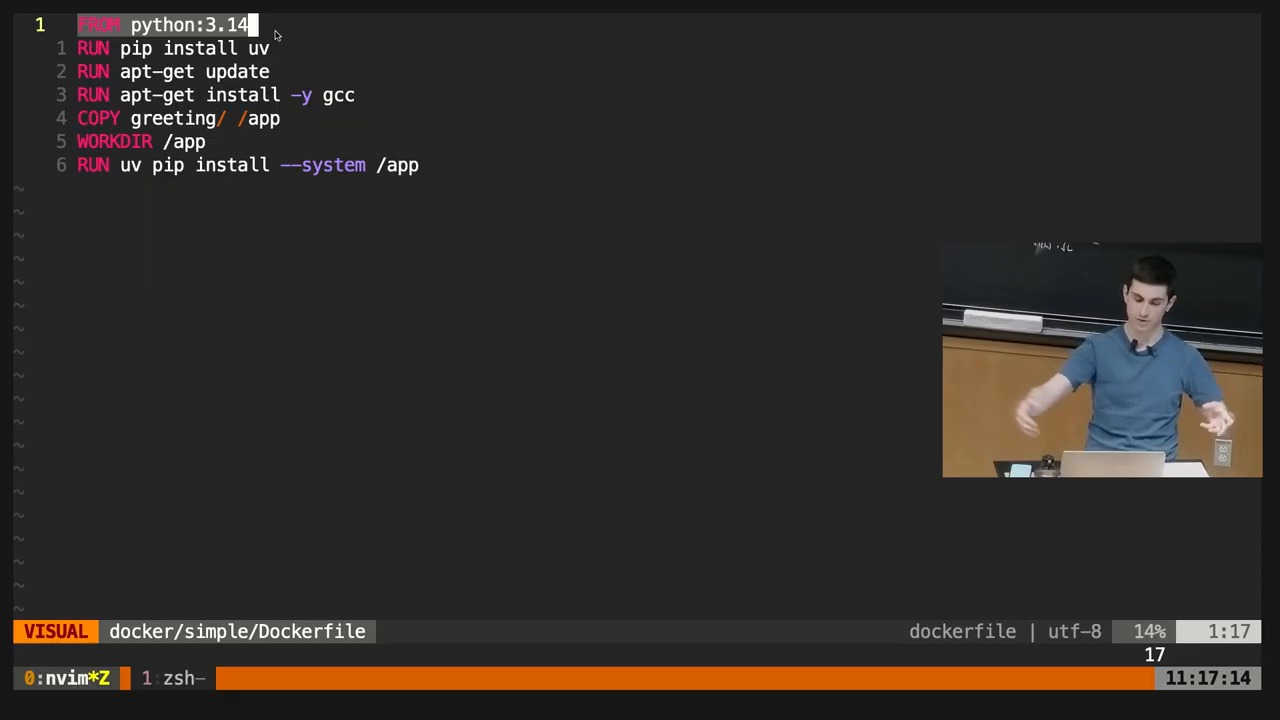
\includegraphics[width=0.92\textwidth]{figures/fig_24_dockerfile.jpg}
\caption{从 python:3.14 出发，安装 uv 和 gcc，复制代码并安装 greeting 的 Dockerfile\vtag}
\end{figure}
\srcnote{00:39:00--00:39:15}
\end{minipage}


现在的问题是：怎样构建自己的镜像？有 Python 镜像不错，但没那么有用，我们想把整个 \texttt{greeting} 库打包进去。为此要使用 Dockerfile 语法。讲者说它看起来像 bash，每条命令都像，但实际上是另一种专门用来创建 Docker 镜像的语言。这里我们说：从 Python 3.14 镜像开始，这是起始文件系统；然后安装 \texttt{uv}；也许需要 C 编译器来构建某些东西；然后复制库需要的文件；最后要安装它，否则这个虚拟计算机里就没有这个包。

\begin{lstlisting}[language=bash]
FROM python:3.14
RUN pip install uv
RUN apt-get update
RUN apt-get install -y gcc
COPY . /app
WORKDIR /app
RUN uv pip install --system /app
\end{lstlisting}

\noindent\begin{minipage}{\textwidth}
\begin{figure}[H]
\centering
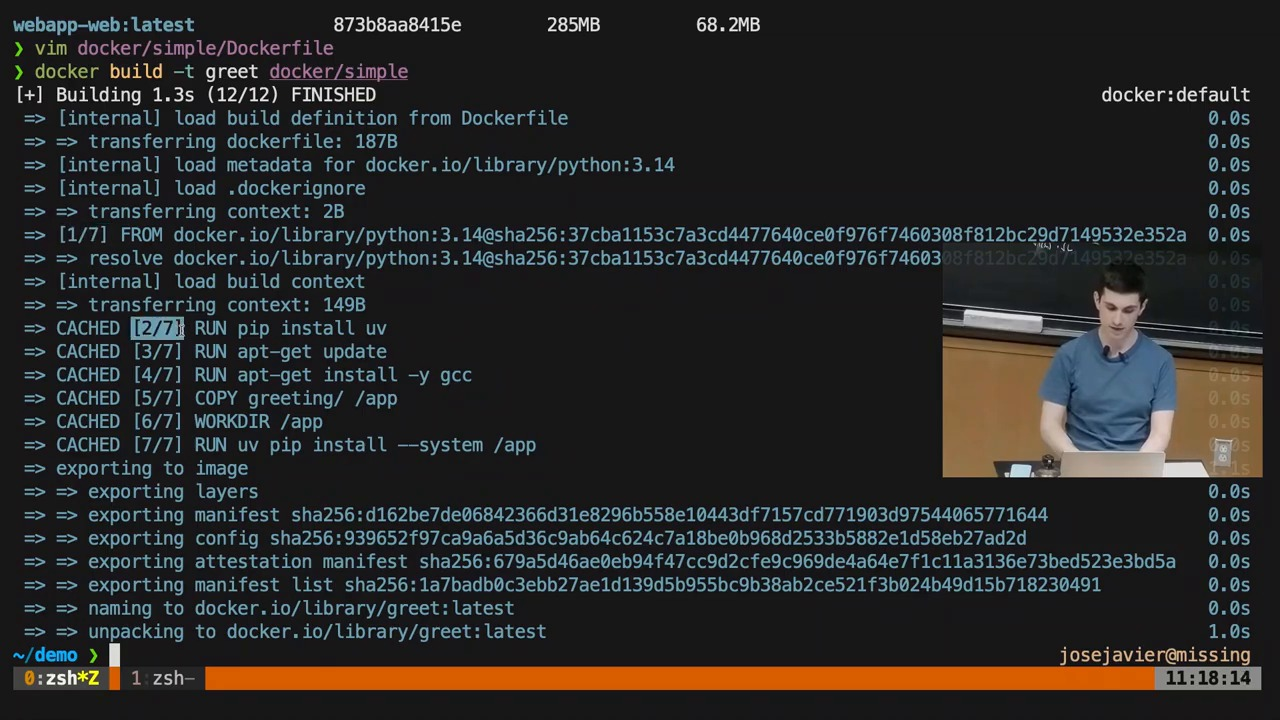
\includegraphics[width=0.92\textwidth]{figures/fig_25_docker_build.jpg}
\caption{\texttt{docker build} 逐条执行指令并为每一步生成一个镜像层\vtag}
\end{figure}
\srcnote{00:40:00--00:40:15}
\end{minipage}


要生成镜像，执行 \texttt{docker build -t greet .}：指向包含 Dockerfile 的文件夹，并给它起个名字，之后就能引用它。构建时它复用了很多步骤，你会看到生成了一串编号，因为 Docker 跟踪每一条命令，为文件系统的变化创建层（layer），以便复用；不同镜像使用相同的层时，可以去重。没有给标签时默认标为 \texttt{latest}，这是约定。由于我们安装了定义 \texttt{greet} 工具的包，并且告诉了 Python 去哪里找，执行 \texttt{docker run greet greet} 就很快地启动了一个带有这个文件系统（包括我们的包）的容器，并执行了那个小小的问候程序。

\subsection{优化镜像}

\noindent\begin{minipage}{\textwidth}
\begin{figure}[H]
\centering
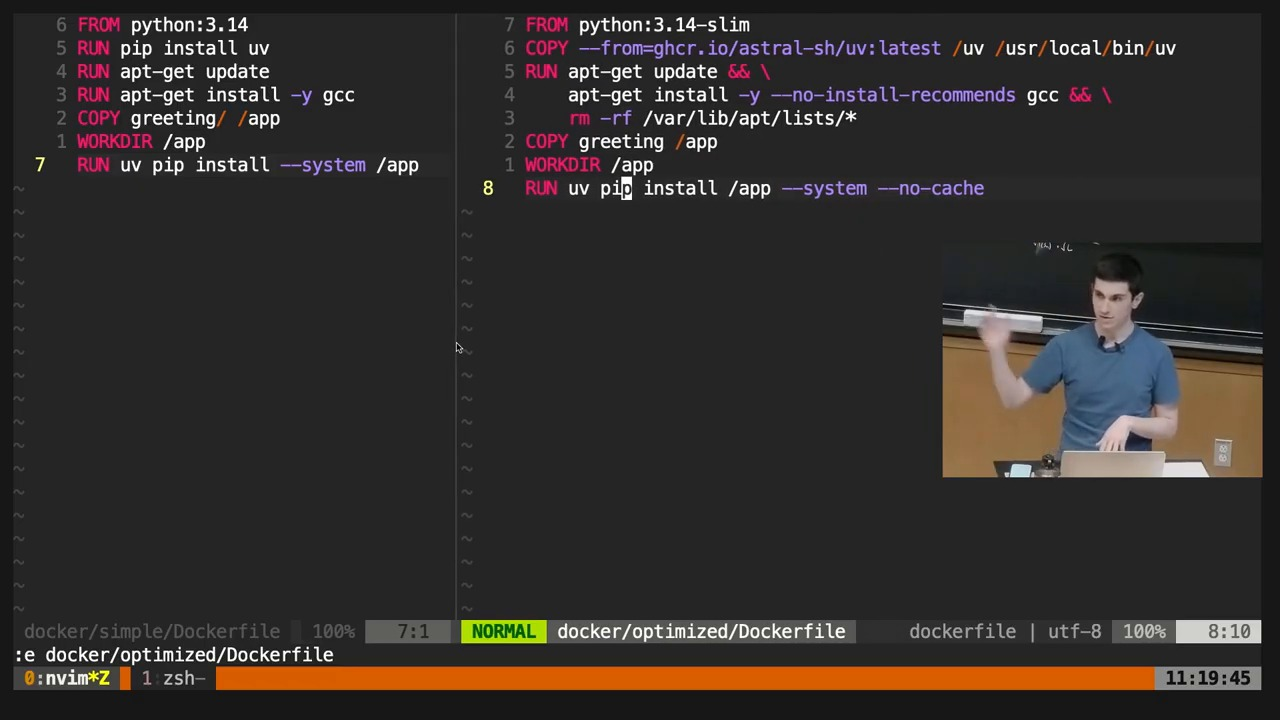
\includegraphics[width=0.92\textwidth]{figures/fig_26_dockerfile_opt.jpg}
\caption{左右对比：优化后的 Dockerfile 改用 slim 基础镜像并合并命令、关闭缓存\vtag}
\end{figure}
\srcnote{00:41:30--00:41:45}
\end{minipage}


讲者说，你可能想直接用写 Shell 脚本的习惯写 Dockerfile，但 Dockerfile 有一些讲究，需要一定的学习过程，实践中最后往往更像右边那样。因为每一步都会创建一个中间层，我们要尽可能减少层。比如 \texttt{apt update} 下载系统包管理器的最新索引，这里把多个操作合并在一起，并给出一些特殊参数：不要保留额外的簿记文件，我们不需要，不会再装别的东西，这是最终产品；对 \texttt{uv} 也一样，不要保存缓存，缓存对一个供人使用的最终镜像没有用处。

\begin{lstlisting}[language=bash]
FROM python:3.14-slim
COPY --from=ghcr.io/astral-sh/uv:latest /uv /bin/uv
RUN apt-get update && \
    apt-get install -y --no-install-recommends gcc && \
    rm -rf /var/lib/apt/lists/*
COPY . /app
WORKDIR /app
RUN uv pip install --system --no-cache /app
\end{lstlisting}

\noindent\begin{minipage}{\textwidth}
\begin{figure}[H]
\centering
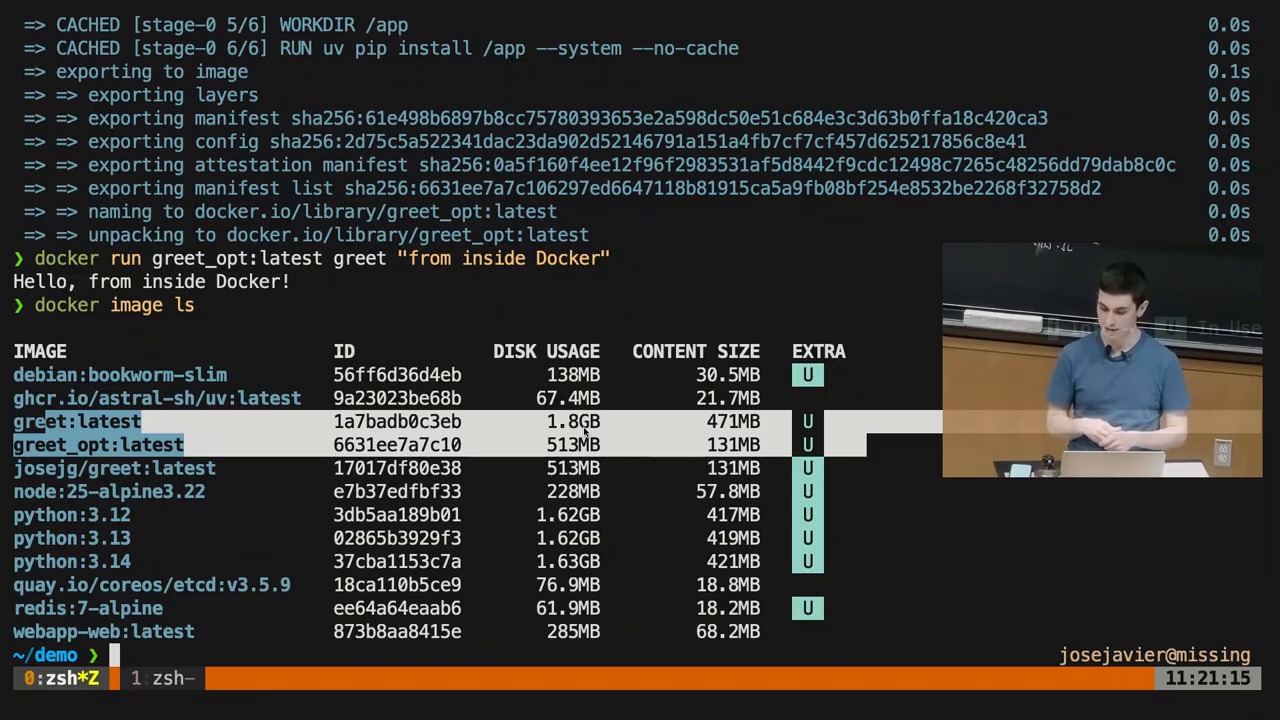
\includegraphics[width=0.92\textwidth]{figures/fig_27_image_sizes.jpg}
\caption{\texttt{docker images} 显示 greet 接近 2GB，而 greet-optimized 约为 0.5GB\vtag}
\end{figure}
\srcnote{00:43:00--00:43:15}
\end{minipage}


构建并运行优化后的镜像，效果一样。区别在于镜像大小。用 \texttt{docker images} 列出镜像，比较未优化的 \texttt{greet} 与优化后的版本：第一个只是下载所有文件、完全不考虑空间，产出的制品接近 2 GB；遵循了这些常见模式的优化版只有大约半 GB。讲者说肯定还能做更多事让它更小、更便于部署。

\begin{warningbox}{示例 Dockerfile 的细节}
讲义作者提醒：上面两段 Dockerfile 根据屏幕内容和讲解整理，细节（例如 \texttt{uv} 的安装方式）可能与讲者的文件不完全一致。原则是确定的：每条 \texttt{RUN} 产生一层，在同一条 \texttt{RUN} 里安装并清理，清理才真正减小镜像；把很少变化的步骤放在前面、经常变化的 \texttt{COPY} 放在后面，才能最大限度利用构建缓存。
\end{warningbox}

\subsection{Dockerfile 是谁写的}

有同学问 Dockerfile 里该写什么，是自己写还是自动生成的。讲者说 Dockerfile 不会自动生成，绝大多数情况下是手写的。过程是弄清你的程序或应用需要什么才能运行。在这个例子里其实可能不需要 C 编译器，可以简化为复制应用源码再安装；他加上它只是为了展示安装和清理的一些惯例。如果 Python 包有需要编译的 C 扩展，那 GCC 就是必需的。在某种程度上，Dockerfile 里该放什么是显而易见的：随着你使用应用、弄清依赖，很快就会意识到“没有这个或那个我的应用就跑不起来”。回到 CuPy，我们知道它需要 CUDA，所以要么从一个提供 CUDA 的镜像开始，要么在 Dockerfile 里设法安装它。

\section{多服务应用与服务管理}

\subsection{依赖整个服务}

\noindent\begin{minipage}{\textwidth}
\begin{figure}[H]
\centering
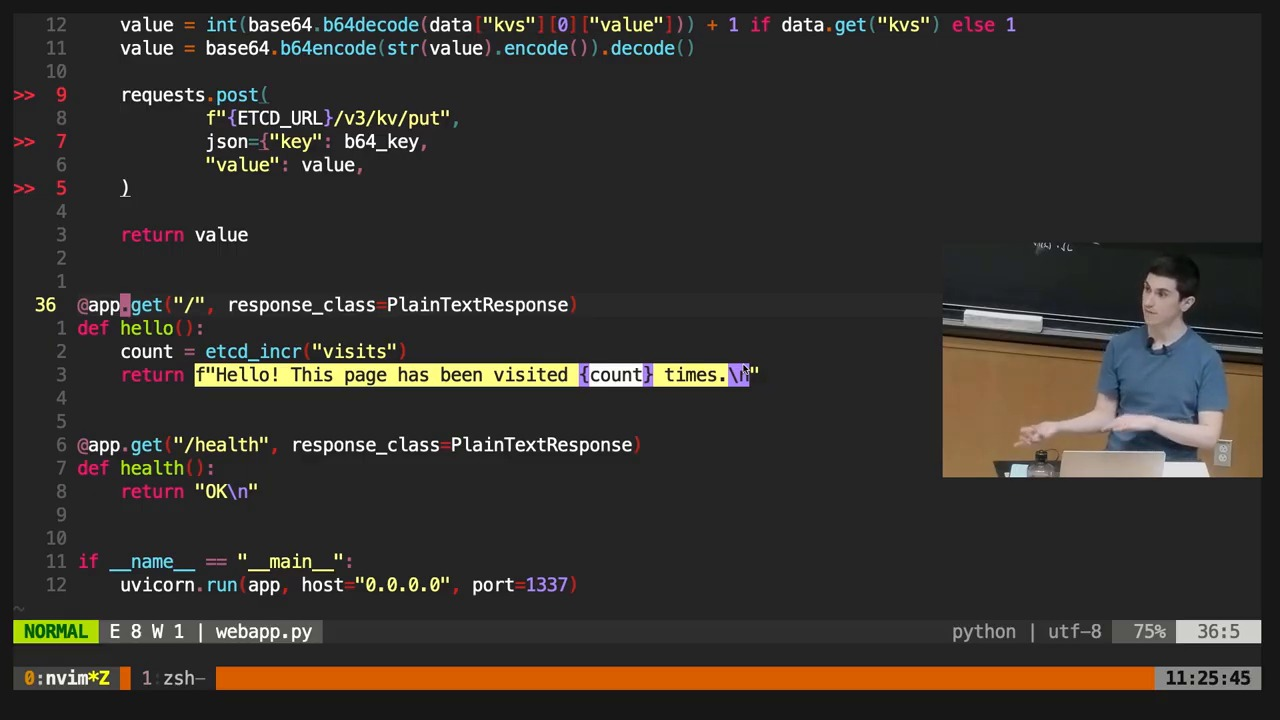
\includegraphics[width=0.92\textwidth]{figures/fig_28_webapp.jpg}
\caption{访问计数 Web 应用：每次访问都通过 HTTP 请求让 etcd 中的计数加一\vtag}
\end{figure}
\srcnote{00:47:30--00:47:45}
\end{minipage}


讲者说，写容器之后会遇到另一层抽象：你依赖的不再是 \texttt{import requests} 那样的普通包，而是整个服务，这些服务有各自独立的容器。比如数据库：如果你使用一整个 PostgreSQL，你可以尝试把 Postgres 装进自己的 Dockerfile，祈祷 Postgres 的依赖和你程序的依赖不冲突；或者把它们分到不同的容器里，让它们相互通信。依赖地狱是真实存在的，协调版本相当复杂，所以第二种模式出现得多得多。

他构造了一个很简单的 Web 应用：每次有人访问，就显示“这个页面被访问了多少次”。当然可以把计数存在文件里，但部署一个真正的数据库更有意思，尤其是一个具有良好性质的数据库。这里用的是 etcd，一个容错、相当健壮的数据库，但它有一些要求，和应用装在一起可能比较麻烦。所以应用通过请求与它通信：每次有人访问网站，就调用一个增加访问计数的辅助函数。由于要编码解码，有一些额外开销，但关键是我们向某个 URL 发送带特定负载的请求：取出键值、加一、再把新值写回。这是最简单的数据库操作，读、写、加一。

\subsection{Docker Compose}

\noindent\begin{minipage}{\textwidth}
\begin{figure}[H]
\centering
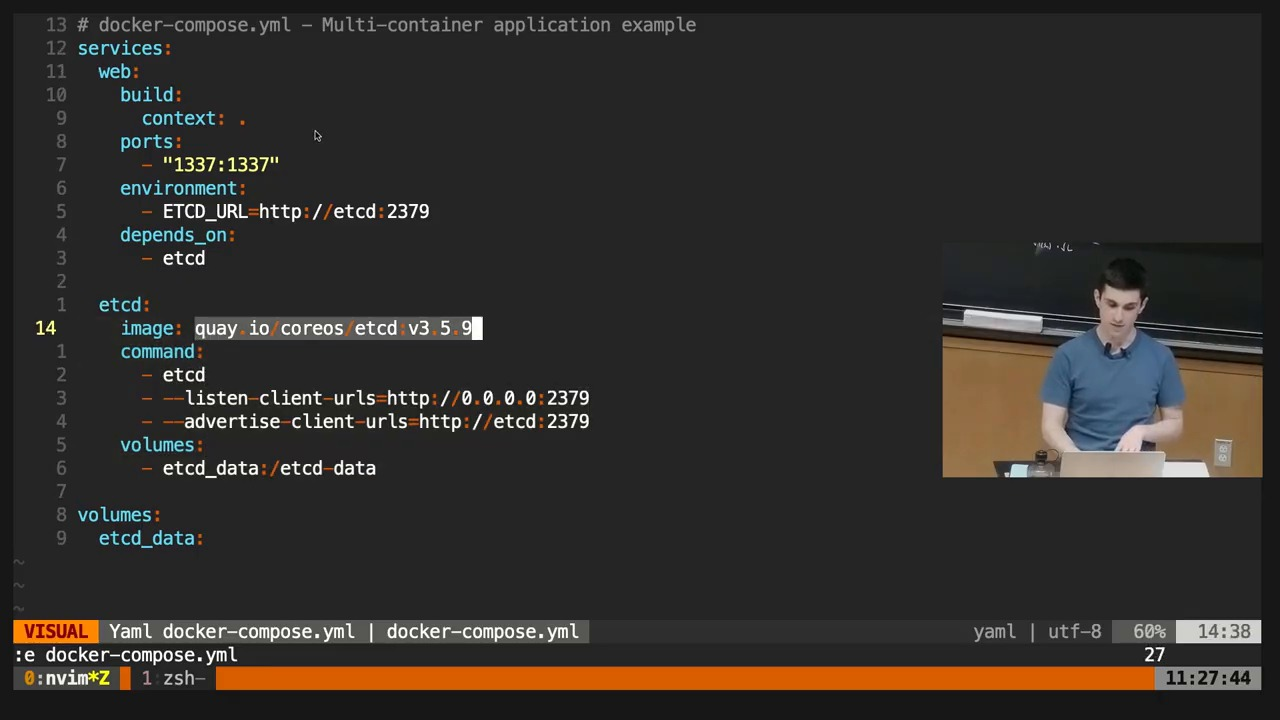
\includegraphics[width=0.92\textwidth]{figures/fig_29_compose.jpg}
\caption{docker-compose.yml 声明 web 与 etcd 两个服务，web 通过 depends\_on 等待数据库\vtag}
\end{figure}
\srcnote{00:49:30--00:49:45}
\end{minipage}


现在问题来了：要部署这两个容器并让它们互相通信。可以用一堆 \texttt{docker run} 命令，还得了解 Docker 网络、让它们处在同一个网络里；但实践中你会看到一种专门的语言，用来描述服务怎样部署和相互连接。Docker Compose 是 Docker 的一个扩展，它读取一个配置文件，把它翻译成一系列 Docker 命令来部署需要的容器。这里部署两个服务：我们的 Web 服务和数据库。数据库直接指定镜像；应用这边有自己的 Dockerfile，所以用另一种写法。讲者特别指出可以声明依赖：数据库运行之前不要启动 Web 服务。手动做这件事可能相当麻烦，这里用声明式的方式就很容易表达。

\begin{lstlisting}[language=bash]
services:
  web:
    build: .
    ports:
      - "5000:5000"
    environment:
      - ETCD_URL=http://etcd:2379
    depends_on:
      - etcd
  etcd:
    image: quay.io/coreos/etcd:v3.5.0
    command: >
      etcd --listen-client-urls http://0.0.0.0:2379
      --advertise-client-urls http://etcd:2379
\end{lstlisting}

\subsection{配置与代码分离}

讲者说，除了打包代码，还要考虑别人怎样运行代码、怎样修改它的行为。一个好的思维模型是：同一个应用应该能部署到两台不同的机器上，只改配置文件，从不修改源代码。比如只是改变监听的端口，就不应该改源代码。配置有多种方式，在脚本那一讲已经见过，其中几种模式在这里再次出现：我们的程序从环境变量 \texttt{ETCD\_URL} 读取数据库的地址，而 etcd 更方便用命令行参数传选项，这里就是这样指定的。

\noindent\begin{minipage}{\textwidth}
\begin{figure}[H]
\centering
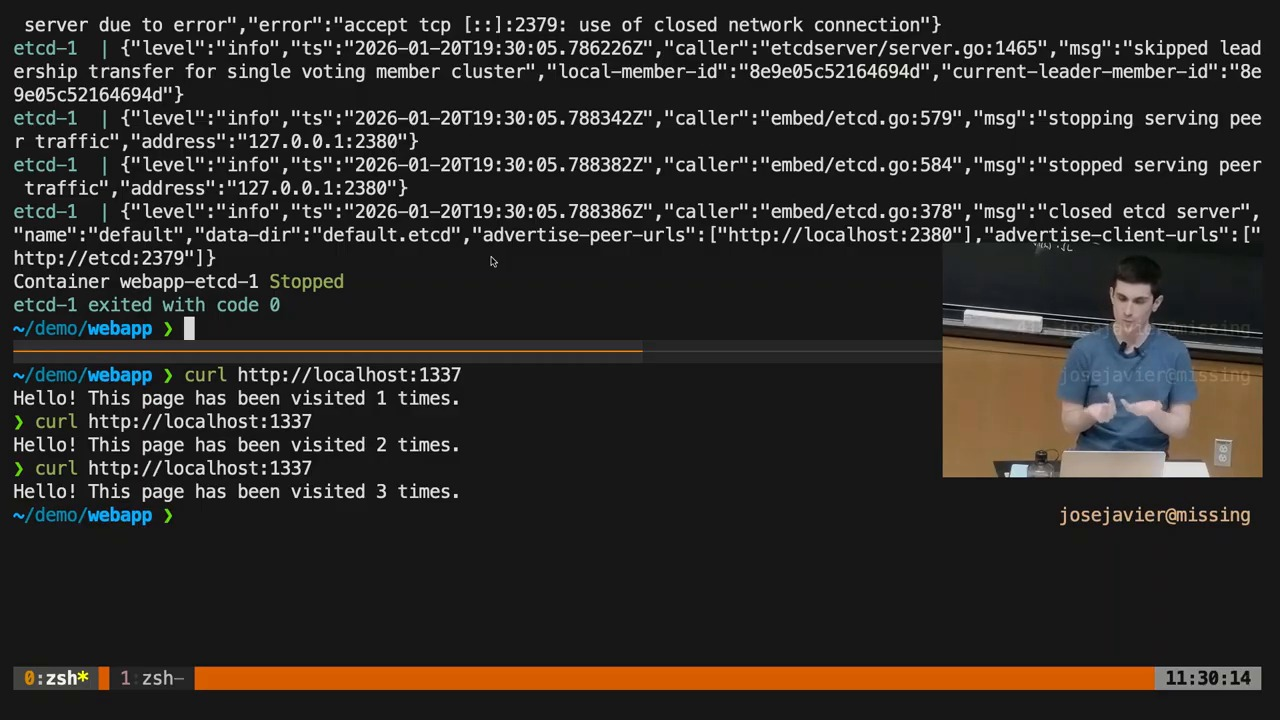
\includegraphics[width=0.92\textwidth]{figures/fig_30_compose_up.jpg}
\caption{\texttt{docker compose up} 启动两个容器，反复 curl 时访问次数依次增加\vtag}
\end{figure}
\srcnote{00:52:00--00:52:15}
\end{minipage}


执行 \texttt{docker compose up}，两个容器都启动了，日志里能看到 etcd 容器和 Web 应用容器，后者说它在某个 URL 上运行。查询这个 URL，得到“页面被访问了 1 次”，再访问是 2 次、3 次，以此类推。每次请求 Web 应用，它都与数据库应用通信来更新计数。这样我们就解决了怎样部署这类更复杂的多服务应用的问题。

\begin{knowledgebox}{配置的常见来源}
讲义作者补充：配置通常按优先级来自命令行参数、环境变量、配置文件和默认值。容器化应用尤其偏爱环境变量，因为同一个镜像可以在开发、测试、生产环境中原封不动地使用，只是注入不同的变量。密码、令牌等敏感信息也不应写进镜像或代码仓库。
\end{knowledgebox}

\subsection{systemd：让服务开机自启}

\noindent\begin{minipage}{\textwidth}
\begin{figure}[H]
\centering
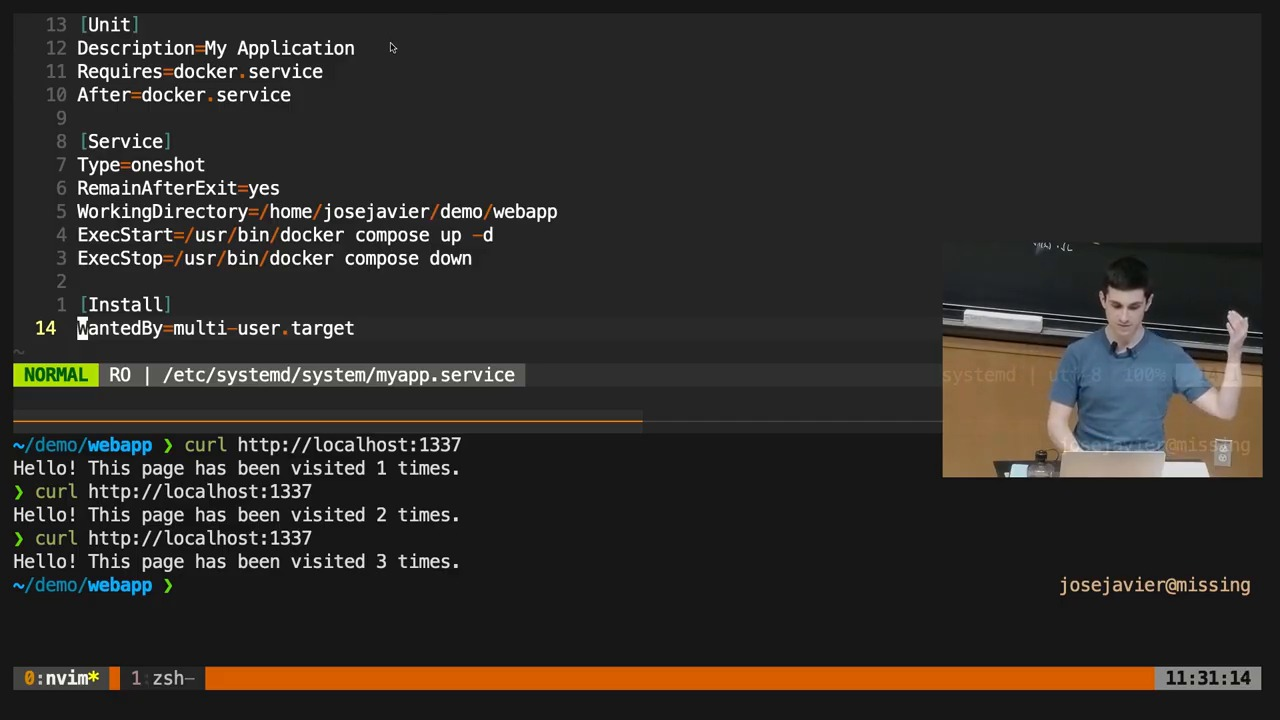
\includegraphics[width=0.92\textwidth]{figures/fig_31_systemd.jpg}
\caption{放在 /etc/systemd/system 下的单元文件：依赖 docker.service，启动时执行 docker compose up -d\vtag}
\end{figure}
\srcnote{00:53:00--00:53:15}
\end{minipage}


还剩一个问题：谁来启动它？总不能指望机器每次重启后都有人 SSH 进来执行 \texttt{docker compose up}。所以另一个常见模式是编排服务的启动方式。Linux 上最流行的是 systemd，它有一种定义服务的方式：在 \texttt{/etc/systemd/system} 下创建一个文件就能注册新服务。它是声明式的，但有自己的语法。讲者说这正是 LLM 非常有用的地方：可以问它有哪些选项，它会教你这种专门的语法。

\begin{lstlisting}[language=bash]
[Unit]
Description=My Application
Requires=docker.service
After=docker.service

[Service]
Type=oneshot
RemainAfterExit=yes
WorkingDirectory=/opt/myapp
ExecStart=/usr/bin/docker compose up -d
ExecStop=/usr/bin/docker compose down

[Install]
WantedBy=multi-user.target
\end{lstlisting}

概括地说，我们告诉宿主 Linux 系统：每次启动时有这样一个应用；请不要在 Docker 服务之前运行它，因为它需要 Docker 服务器在运行；进入这个文件夹，执行 \texttt{docker compose up -d}，\texttt{-d} 表示分离运行，不挂在命令行上；需要停止时执行 \texttt{docker compose down}。

\noindent\begin{minipage}{\textwidth}
\begin{figure}[H]
\centering
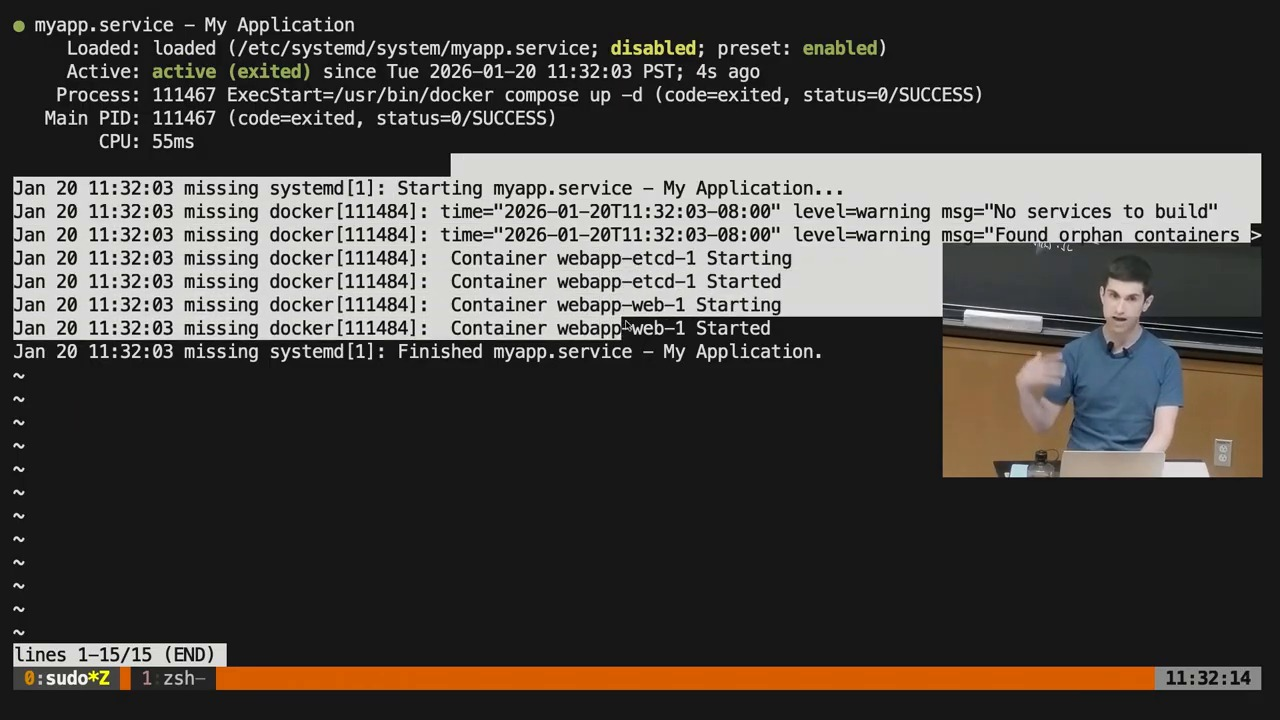
\includegraphics[width=0.92\textwidth]{figures/fig_32_systemd_status.jpg}
\caption{\texttt{systemctl status} 显示服务已由 systemd 启动，日志里是 docker compose 的输出\vtag}
\end{figure}
\srcnote{00:54:00--00:54:15}
\end{minipage}


用 \texttt{systemctl} 命令行工具启动服务，它根据这个文件来操作。启动后看起来什么都没发生，但查看状态就能看到，之前手动执行 \texttt{docker compose up} 做的事已经完成了，只是现在由操作系统来管理，机器重启后它会自动启动。再访问那个网站，它又在运行了，显示被访问了 4 次。要停止，只需停止这个服务。

\begin{practicebox}{动手试一试}
讲义作者整理：把上面的 Compose 文件与一个最小的 Flask 应用放在同一目录，执行 \texttt{docker compose up}，用 \texttt{curl} 访问几次；然后执行 \texttt{docker compose down} 再重新启动，观察计数是否保留，并思考 etcd 的数据存放在哪里、怎样用卷（volume）让它持久化。
\end{practicebox}

\subsection{本章小结}

依赖整个服务时，把每个服务放进自己的容器，用 Docker Compose 声明它们的连接和启动顺序；配置通过环境变量和参数注入而不改代码；systemd 负责让整套服务随系统启动。

\section{发布制品}

\subsection{从网站和 GitHub 安装}

\noindent\begin{minipage}{\textwidth}
\begin{figure}[H]
\centering
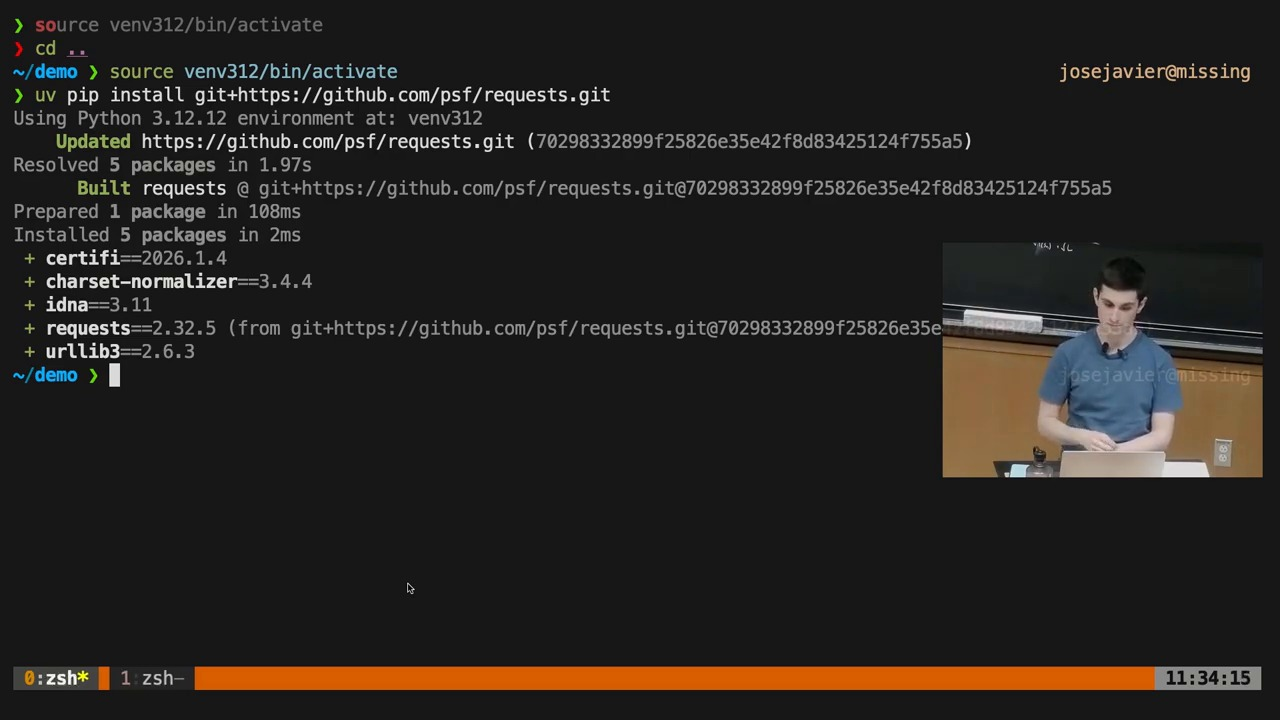
\includegraphics[width=0.92\textwidth]{figures/fig_33_pip_github.jpg}
\caption{pip 可以直接从 GitHub 仓库或某个发布版本的 wheel 地址安装\vtag}
\end{figure}
\srcnote{00:56:00--00:56:15}
\end{minipage}


讲者说最后一个主题是怎样让人获取这些制品。到目前为止我们一直在创建文件，可文件放在哪里？可以放在网站上让人下载，比如 Ubuntu 就是这么做的。但实践中常见的方式，如我们一直看到的，是放在 GitHub 上：很多包把代码放在 GitHub 并给出安装说明。事实上包管理器可以直接从 GitHub 安装：之前我们 \texttt{pip install requests} 是去 PyPI，但也可以从最新版本的源代码安装，这会下载源码、从中构建 wheel、再安装 wheel。还可以看 \texttt{requests} 是否发布了 wheel，它确实发布了，于是可以复制那个 URL 安装，这次不是从最新版本，而是从某个特定发布版本安装。它只是一个文件，只要能拿到就能安装。

\begin{lstlisting}[language=bash]
uv pip install git+https://github.com/psf/requests.git
uv pip install https://github.com/psf/requests/releases/download/v2.32.5/requests-2.32.5-py3-none-any.whl
\end{lstlisting}

那 \texttt{pip} 平时去哪里下载？可以让它输出全部信息，再过滤出 wheel 一行。先卸载再重新安装，就能看到获取元数据用的确切 URL，以及获取包本身用的 URL。

\begin{warningbox}{示例 URL 仅供示意}
讲义作者提醒：上面第二条命令中的版本号和文件名是讲义作者按 GitHub 发布页的命名规则补写的示例，实际使用时请到项目的 releases 页面复制真实存在的地址。
\end{warningbox}

\subsection{发布到 PyPI}

\noindent\begin{minipage}{\textwidth}
\begin{figure}[H]
\centering
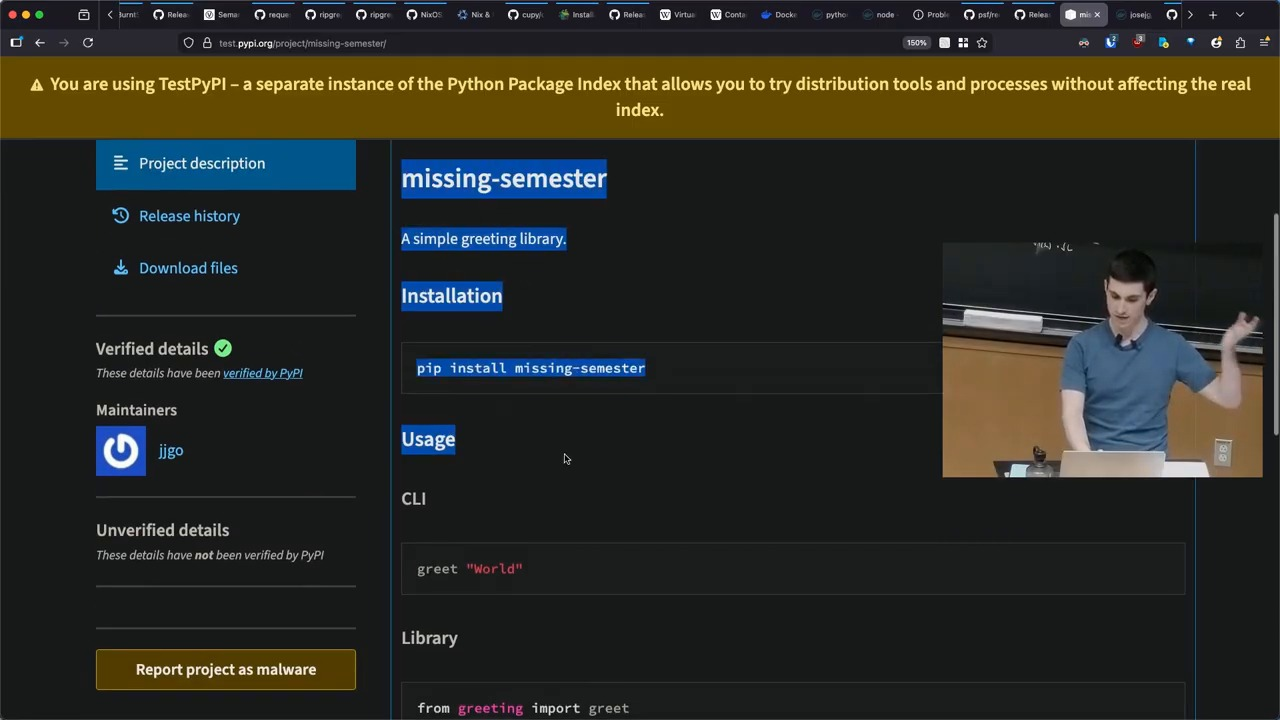
\includegraphics[width=0.92\textwidth]{figures/fig_34_uv_publish.jpg}
\caption{用 \texttt{uv publish} 上传后，missing-semester 包出现在 TestPyPI 上\vtag}
\end{figure}
\srcnote{00:58:30--00:58:45}
\end{minipage}


现在的问题是：怎样把自己的包放到 PyPI 上，让别人找到？\texttt{pip} 帮不了这个忙，\texttt{uv} 可以。\texttt{greeting} 这个名字已经被占用了，所以讲者用 \texttt{missing-semester} 包来演示：构建包，得到 wheel，再执行 \texttt{uv publish}，附带一个额外参数，就把 wheel 上传到包索引供别人使用。他解释了那个参数：随便上传会污染 PyPI，所以 Python 开发者做了 TestPyPI，它是 PyPI 的一个副本，可以用来测试怎样发布包。页面上能看到之前测试的版本，刚才这次上传把它升到了下一个修订版本；因为提供了说明，页面上还有 README 供人阅读。再从 TestPyPI 执行 \texttt{uv pip install missing-semester}，就下载并解压到了虚拟环境中。

\begin{lstlisting}[language=bash]
uv build
uv publish --publish-url https://test.pypi.org/legacy/
uv pip install --index-url https://test.pypi.org/simple/ missing-semester
\end{lstlisting}

\subsection{发布 Docker 镜像}

\noindent\begin{minipage}{\textwidth}
\begin{figure}[H]
\centering
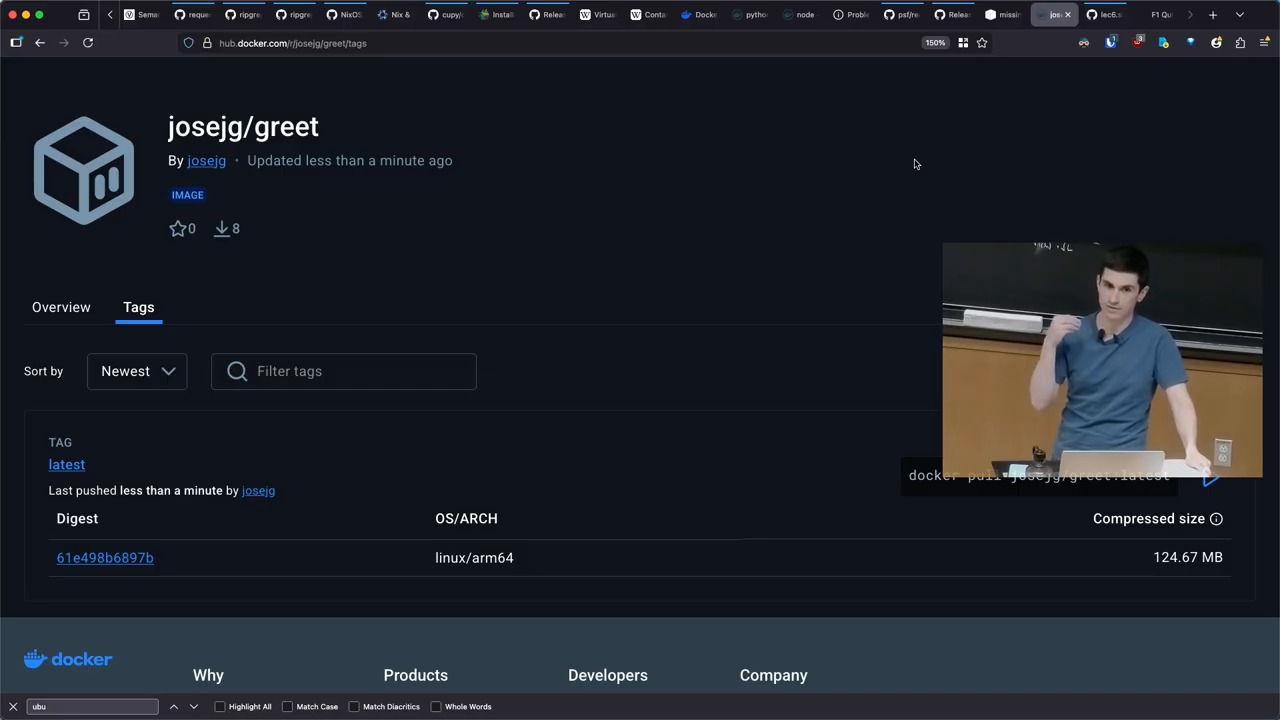
\includegraphics[width=0.92\textwidth]{figures/fig_35_docker_hub.jpg}
\caption{推送到 Docker Hub 后，jjgo/greet 镜像对所有人可见\vtag}
\end{figure}
\srcnote{01:00:30--01:00:45}
\end{minipage}


讲者说，几乎任何包的流程都很相似，Docker 之类也一样。要发布镜像供人使用，先要以特定方式构建：Docker 只允许把镜像推送到有权限的仓库，他只能推送以自己用户名开头的镜像，所以要按这个要求重新打标签。镜像和之前构建的完全一样，所以这一步几乎什么都不做，只是打标签。推送时 Docker 发现所有层之前都推送过了。到 Docker Hub 上查看，任何人都可以下载这个镜像，得到一个运行 \texttt{greet} 应用的完整文件系统。

\begin{lstlisting}[language=bash]
docker build -t jjgo/greet .
docker push jjgo/greet
\end{lstlisting}

\subsection{答疑：怎样与同伴共享镜像}

讲者最后说，习题覆盖了很多这样的模式，信息量很大，很多要靠动手学：自己写 \texttt{pyproject.toml}、写 Dockerfile、推送和安装。希望今天的内容给大家一个好的思维框架，理解依赖以及现代软件应用怎样构建和在网上分发。

有同学问怎样把镜像分享给同伴。讲者说要使用容器镜像仓库（container registry），就像他刚才推送一样。Docker Hub 不是唯一的镜像仓库，只要你和同伴都能访问同一个地方，就可以 \texttt{docker pull} 和 \texttt{docker push}，镜像包含所有依赖。你需要认证，向 Docker Hub、GitHub 容器仓库或你使用的任何仓库证明你是你、有权读取这个容器的内容，然后就能下载整个镜像并运行应用。同样的思路适用于几乎任何框架，比如 PyPI：有公共的地方，也可以放在 GitHub 上，如我们所见可以直接从那里安装。只要有一个共同的仓库来存放代码或制品，相互协作就很容易。

\section{总结}

\begin{itemize}
\item 代码能运行依赖于一整套隐式条件；打包就是把代码连同它对环境的假设，做成别人能下载运行的制品。
\item 包管理器从包索引递归解析依赖树；每个项目使用独立的虚拟环境，必要时隔离运行时版本，\texttt{uv} 是当前顺手的 Python 工具。
\item \texttt{pyproject.toml} 声明包名、版本、依赖、构建系统和命令行入口；\texttt{uv build} 生成 sdist 与 wheel。
\item 预编译制品受操作系统和 CPU 架构限制，含原生扩展的包还要区分运行时版本。
\item 语义化版本让版本号表达兼容性；库给宽范围，应用钉死版本，锁文件连同哈希记录整棵依赖树；Nix 把可复现性推广到整个系统。
\item 容器共享宿主内核、隔离应用层；Dockerfile 逐层构建镜像，合并命令和清理缓存可以显著缩小镜像。
\item 多服务应用用 Docker Compose 声明，配置通过环境变量和参数注入；systemd 让服务随系统启动。
\item 制品通过 PyPI、GitHub、Docker Hub 等仓库分发，TestPyPI 用来练习发布。
\end{itemize}

\begin{practicebox}{自测}
\begin{enumerate}
\item 为什么在全局 Python 中安装所有项目的依赖迟早会出问题？虚拟环境本质上改变了什么？
\item 一个库的 \texttt{pyproject.toml} 应该写 \texttt{requests==2.32.3} 还是 \texttt{requests>=2.0,<3}？一个应用呢？
\item 版本从 1.4.2 升到 2.0.0、1.5.0、1.4.3，按语义化版本各意味着什么？
\item 锁文件里为什么要记录哈希，而不只是版本号？
\item 容器与虚拟机相比省掉了什么？为什么在 macOS 上运行 Docker 仍然需要虚拟机？
\item 修改上面的 Dockerfile，使只改动源码时不必重新安装依赖。
\end{enumerate}
\end{practicebox}

\end{document}
